
At the time of writing, most of the contents of this chapter are under review, and posted as a
preprint~\citet{visani_hermes_2026}, under the title \textit{HERMES: Holographic Equivariant neuRal
network model for Mutational Effect and Stability prediction}.

This work originated as a re-implementation of the \textit{Holographic-CNN} (H-CNN), developed by my mentor
and former labmate Mike Pun~\citep{pun_learning_2024}. I desired to re-implement the network within
the framework I was familiar with, and that had external support, so that I could better use it and better
tweak it as I saw fit. Following up on Mike's initial findings that H-CNN could be used to predict
the effect of mutations on diverse protein functions, and considering emergent works that used similar
high-level principles as H-CNN to predict mutation effects, I ventured to improve upon H-CNN with the goal
of mutation effect prediction in mind. These efforts resulted not only in a new family of models - the
HERMES models - but also in a systematic analysis of the strengths, weaknesses and differences among
models in the "machine learning for protein mutation effect" literature.

Starting with biological motivations, understanding the effects of amino acid substitutions on protein
function is fundamental to biological discovery and engineering, with applications spanning disease
variant identification~\citep{gerasimavicius_identification_2020,blaabjerg_rapid_2023}, enzyme optimization
and engineering~\citep{ishida_effects_2010,wang_d3distalmutation_2021}, viral escape
prediction~\citep{thadani_learning_2023,Luksza2014-pg,Neher2014-pf}, antibody
engineering~\citep{hie_efficient_2024}, and vaccine antigen
stabilization~\citep{mclellan_structure-based_2013, gonzalez_general_2024, bakkers_efficacious_2024,
milder_universal_2022, phan_conserved_2022}.

Mutational effects on thermodynamic stability and binding affinity are particularly well-studied, as
stability is typically prerequisite for function~\citep{rocklin_global_2017} and most biological
processes are mediated by binding events. While these effects can be measured experimentally via
denaturation assays~\citep{lindorff-larsen_linking_2021}, surface plasmon
resonance~\citep{karlsson_spr_2004}, or deep mutational
scanning~\citep{fowler_deep_2014,Kinney2019-wc,starr_deep_2020}, such experiments remain laborious
despite recent throughput improvements~\citep{tsuboyama_mega-scale_2023}.

Computational approaches offer an alternative. Molecular dynamics simulations can accurately capture
short-time (nano seconds) responses, but are limited in predicting substantial conformational
changes often induced by mutations~\citep{gapsys_accurate_2016}. Physics-based energy functions,
including FoldX~\citep{schymkowitz_foldx_2005} and Rosetta~\citep{kellogg_role_2011}, remain widely
used to predict mutation-induced stability changes~\citep{gonzalez_general_2024}, yet are often slow
and inaccurate~\citep{blaabjerg_rapid_2023}. In recent years, machine learning models have shown
considerable progress in this area: models trained to predict amino acid propensities at a given
residue from surrounding sequence~\citep{riesselman_deep_2018, meier_language_2021} or structural
context~\citep{pun_learning_2024, diaz_stability_2024, blaabjerg_rapid_2023,
li_predicting_2020,benevenuta_antisymmetric_2021, dieckhaus_transfer_2024} can approximate
mutational effects across phenotypes.

Recent work improves these pre-trained baselines by modifying the pre-training
objective~\citep{gordon_protein_2024,gong_evolution-inspired_2024}, and by fine-tuning to predict
phenotype-specific mutational effects~\citep{dieckhaus_transfer_2024, diaz_stability_2024,
blaabjerg_rapid_2023, luo_rotamer_2022}, with thermodynamic stability as a frequent target for
structure-based models~\citep{dieckhaus_transfer_2024, diaz_stability_2024, blaabjerg_rapid_2023}.
Notable examples include RaSP~\citep{blaabjerg_rapid_2023}, which fine-tunes a 3D convolutional
neural network (CNN) on Rosetta-computed $\Delta\Delta G$ values~\citep{chaudhury_pyrosetta_2010};
Stability-Oracle~\citep{diaz_stability_2024}, a graph transformer fine-tuned on experimental
stability measurement from the Megascale dataset~\citep{tsuboyama_mega-scale_2023}; and
ThermoMPNN~\citep{dieckhaus_transfer_2024}, which fine-tunes the inverse folding model
ProteinMPNN~\citep{dauparas_robust_2022} on a different subset of Megascale.

Here, we present HERMES, a family of structure-based models built upon our previous H-CNN
architecture~\citep{pun_learning_2024}. Like H-CNN, HERMES employs a 3D rotationally equivariant,
all-atom CNN architecture, but incorporates implementation improvements yielding a $\sim 2.75\times$
speedup and an adaptable architecture enabling fine-tuning for arbitrary downstream tasks. We first
pre-train HERMES on an inverse folding objective (i.e., predicting a residue's amino acid identity
from its surrounding atomic neighborhood within a 10 \AA~radius), then fine-tune for predicting
mutational effects. The HERMES family comprises three model variants that differ in their treatment
of structural context: HERMES-{\em fixed}, which holds the local environment static during
prediction; HERMES-{\em relaxed}, which enables local structure relaxation through explicit
side-chain repacking; and HERMES-{\em amortized}, which implicitly encodes the structural
flexibility associated with different substitutions through amortization. We systematically analyze
the biases of these models with respect to the physicochemical properties of mutating residues and
characterize their utility across different tasks.

On thermodynamic stability benchmarks, we show that fine-tuned HERMES models match or exceed
state-of-the-art performance. However, we identify a ``wild-type preference bias" introduced by the
pre-training objective that is only partially eliminated by fine-tuning. We also demonstrate HERMES'
utility for structure-based vaccine design, where stabilizing viral envelope glycoproteins in their
metastable pre-fusion conformation is essential for presenting neutralizing antibody
epitopes~\citep{mclellan_structure-based_2013}. Identifying stabilizing mutations traditionally
requires domain expertise and costly experimental iteration. While computational approaches using
Rosetta~\citep{gonzalez_general_2024, phan_conserved_2022} or machine learning (e.g.,
ReCAP~\citep{bakkers_efficacious_2024}) have emerged, HERMES offers significant computational
efficiency over Rosetta and, unlike ReCAP, is publicly available.
When evaluated on 33 known
stabilizing mutations across 5 viral envelopes, HERMES ranks 19 within the top 3 predicted
substitutions at each position, with particularly strong performance on mutations that stabilize
independently without synergistic interactions.
\GM{We also illustrate two mutation discovery pipelines using full saturation mutagenesis with HERMES
to suggest an initial set of candidates, followed by a refinement of the candidate set with Rosetta.}
Lastly, we demonstrate that HERMES can be fine-tuned
to predict mutational effects on protein-protein binding affinity, benchmarking competitively
against existing models.

Code is open source at \url{https://github.com/StatPhysBio/hermes/tree/main}.




\begin{figure}[ht!]
    \centering
    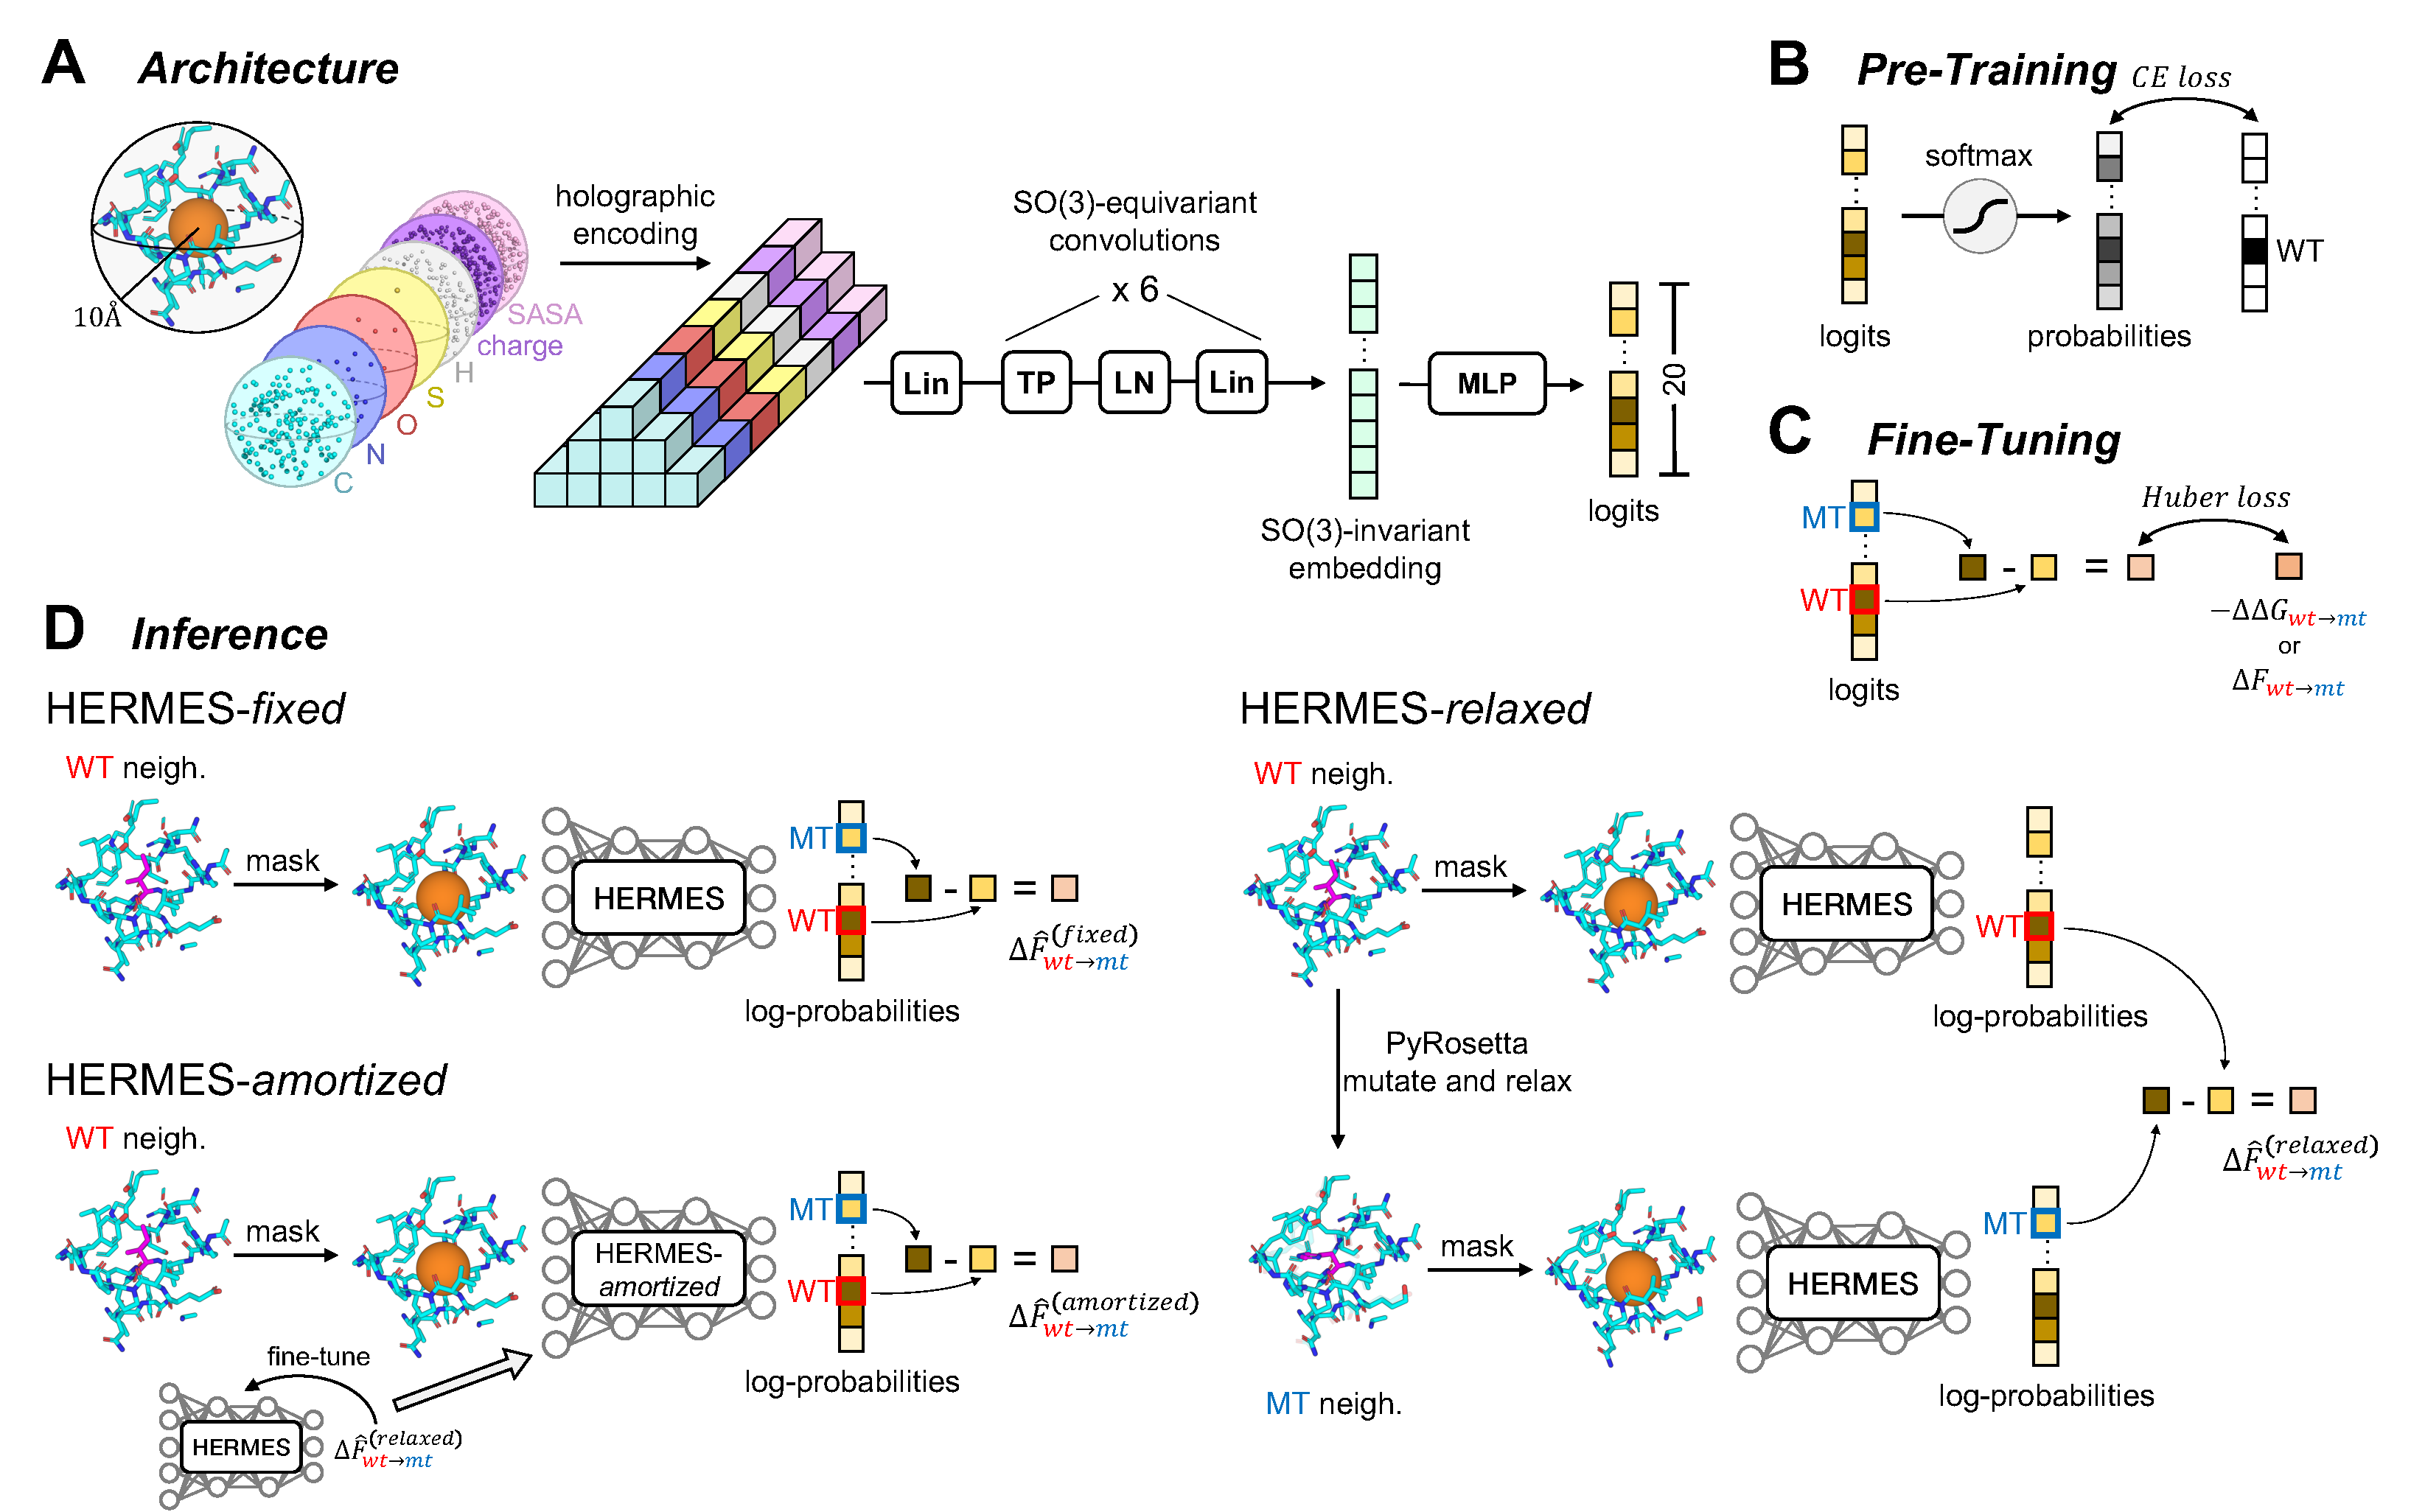
\includegraphics[width=1.0\linewidth]{figures/hermes_with_inference.pdf} \figcaption{Overview of
    HERMES.}{
    \textbf{(A)} Model architecture: HERMES takes as input an all-atom structural neighborhood
    (10~\AA{} radius) around a masked focal residue. Each atom is represented by its 3D coordinates,
    element type, partial charge, and solvent-accessible surface area (SASA). The neighborhood is
    projected onto a Zernike Fourier basis (spherical hologram) and processed by {rotation (SO(3))}
    equivariant layers to produce a rotation-invariant embedding, which is mapped to 20
    amino-acid-specific logits (Methods).\textbf{(B)}
    Pre-training: models are trained to predict the identity of the masked focal residue from its
    surrounding {atomic} neighborhood; logits in (A) are converted to amino-acid propensities
    (probabilities) via a softmax. \textbf{(C)}
    Fine-tuning for mutational effects: model weights are optimized to regress the logit difference
    between mutant and wild-type amino acids to the {corresponding} experimental mutational effect.
    \textbf{(D)} Inference protocols. HERMES-{\em fixed} scores a substitution as the difference
    between the the mutant and wild-type amino-acids logits from a single forward pass, conditioned
    on the masked wild-type neighborhood $X_\wt$. HERMES-{\em relaxed} conditions the mutant term on
    an approximate mutant neighborhood $\hat X_{\wt\to\mt}$ generated in-silico by introducing the
    mutation on the wild-type structure and locally relaxing the structure {with}
    Rosetta~\citep{chaudhury_pyrosetta_2010}. {HERMES-{\em amortized}} distills the relaxed protocol
    by fine-tuning on HERMES-{\em relaxed} predictions, enabling fast fixed-style inference while
    retaining relaxation-aware behavior.}
    \label{fig:HERMES}
\end{figure}


\section{Methods}

\noindent{\bf HERMES architecture and pre-training on masked amino acid classification.}

At its core, HERMES is a 3D, rotationally equivariant convolutional neural network that predicts the propensity
of the 20 different canonical amino acids at a masked (removed) {focal} residue, given its local
atomic neighborhood within the protein structure (Fig.~\ref{fig:HERMES}A).

Atomic neighborhoods - centered at the focal residue's C$\alpha$ and with radius 10~\AA~- are 
first featurized by atom type (including added hydrogens), partial charge,
and solvent-accessible surface area, and then encoded into \textit{holograms} via the ZFT
(Eq.~\ref{eq:ZFT}). Then, a stack of SO(3)-equivariant layers - shown in Fig.~\ref{fig:HERMES}A and detailed
in Section~\ref{sec:layers} - map this encoding to a
rotation-invariant embedding, which a final MLP converts into amino-acid propensities.

For pre-training, we train HERMES to recover the identity of the masked residues on ProteinNet's
CASP12 set, filtered at 30\% sequence identity~\citep{alquraishi_proteinnet_2019}
(Fig.~\ref{fig:HERMES}B). Each model is an ensemble of 10 independently trained networks (3.5M
parameters each), with predictions averaged at inference. To improve robustness for zero-shot
applications, we additionally train models with 0.50~\AA~coordinate noise. Pre-training performance
is summarized in Table~\ref{table:aa_wt_cls}. See Extended Methods in Appendix~\ref{sec:hermes_appendix}
for further details.


\noindent{\bf Zero-shot prediction of mutational effects with pre-trained HERMES.}
The pre-trained HERMES model outputs $P(aa| X_{i,aa})$, the probability of assigning amino acid $aa$
at residue $i$, given the surrounding atomic environment (neighborhood) $X_{i,aa}$ in the structure.
Crucially, $X_{i,aa}$ depends on the $aa$: the neighborhood geometry has the fingerprint of the
masked amino acid during pre-training.

Conditional models are widely used for zero-shot prediction of mutational effects on protein
function (e.g., \citep{riesselman_deep_2018, meier_language_2021, pun_learning_2024}). We
approximate the effect of wild-type to mutant ($\wt \to \mt$) substitution at residue $i$ by the
log-likelihood ratio between the wild-type and the mutant amino acids, conditioned on the respective
local atomic neighborhoods $X_{i,\wt}$ and $X_{i,\mt}$ (omitting the residue index $i$ for clarity):
\begin{equation}
\begin{aligned}
  \Delta \hat F_{\wt \to \mt}  \propto  \log P(\mt | X_{\mt}) - \log P(\wt | X_{\wt})
\end{aligned}
\label{eq:log_ratio_wt_and_mt}
\end{equation}
Here, the neighborhood $X$ depends on the identity of the original amino acid ($\wt$ or $\mt$),
suggesting the potential need for having access to mutant structures for such predictions. The
$\hat\cdot$ {(hat)} indicates the model-predicted mutational effects, as opposed to experimental
measurements (no hat).

When a mutant structure is unavailable, neighborhoods can be relaxed {\em in silico} (e.g., by
Rosetta~ \citep{chaudhury_pyrosetta_2010}), though this procedure is computationally expensive. A
common alternative is to score all mutations using a single (typically wild-type)
structure~\citep{dauparas_robust_2022,diaz_stability_2024,pun_learning_2024}. Here, we {consider}
both of these protocols: {\bf HERMES-{\em fixed}} evaluates mutational effects using the wild-type
structure only (for both $\mt$ and $\wt$ propensities), while {\bf HERMES-{\em relaxed}} evaluates
the propensity of the mutant amino acid in the Rosetta-relaxed $\mt$ neighborhood $\hat X_{\wt \to
\mt}$ starting from the available $\wt$ structure (Fig.~\ref{fig:HERMES}D); see Methods for details.
The resulting estimates for mutational effects from these two approaches follow,
\begin{equation}
\begin{aligned}
\Delta \hat F_{\wt \to \mt}^{\text{(HERMES-{\em fixed})}} &\propto \log P\left(\mt \mid
X_{\wt}\right) - \log P\left(\wt \mid X_{\wt}\right)\\
\Delta \hat F_{\wt \to \mt}^{\text{(HERMES-{\em relaxed})}} &\propto \log P\left(\mt \mid \hat
X_{\wt \to \mt}\right) - \log P\left(\wt \mid X_{\wt}\right).
\end{aligned}
\label{eq:deltaF_variants}
\end{equation}

\noindent{\bf Fine-tuning HERMES to predict protein function.}
Context-conditioned amino-acid likelihoods provide useful zero-shot proxies for mutational effects
across diverse functions~\citep{riesselman_deep_2018, meier_language_2021, pun_learning_2024}, but
supervised models for specific functions can perform better in practice. Building on prior
work~\citep{blaabjerg_rapid_2023, diaz_stability_2024}, we fine-tune HERMES models directly on
mutational effect data. Unlike approaches that train a separate regression
head~\citep{blaabjerg_rapid_2023, diaz_stability_2024, dieckhaus_transfer_2024}, we update the
model end-to-end so that its \emph{predicted scores} themselves align with measurements.
Specifically, as shown in Fig.~\ref{fig:HERMES}C,
we make the predicted HERMES-{\em fixed} $\Delta \hat F_{\wt \to \mt}^{\text{(HERMES-{\em fixed})}}$
(eq.~\ref{eq:deltaF_variants}) regress over the experimentally measured mutational effects $\Delta
F_{\wt\to \mt}$ by minimizing a robust Huber loss,
\begin{equation}
   \mathcal{L} = \text{HuberLoss}(\Delta \hat F_{\wt \to \mt}^{\text{(HERMES-{\em fixed})}}, \Delta
   F_{\wt \to \mt})
\label{eq:loss_function}
\end{equation}
which stabilizes training under outliers while calibrating predictions to the function of interest.
See Extended Methods in Appendix~\ref{sec:hermes_appendix} for further details.\\


\noindent{\bf Hermes-{\em amortized} to encode structural flexibility in HERMES-{\em fixed} by
amortization.}
Because the structural-relaxation step in HERMES-\emph{relaxed} is computationally costly ($\sim 66$
times slower than HERMES-{\em fixed} on a single CPU / A40 GPU, Table~\ref{table:inference_speed}),
we distill HERMES-\emph{relaxed} predictions into the model via a fine-tuning procedure. Concretely,
we fine-tune the model so that the mutational-effect predictions produced with the fast
HERMES-\emph{fixed} protocol regress to the corresponding HERMES-\emph{relaxed} predictions {via
Eq.~\ref{eq:loss_function}} (Fig.~\ref{fig:HERMES}D). We perform this fine-tuning on a small subset
of neighborhoods extracted from the pre-training proteins ($\sim$15k neighborhoods, 0.5\% of the
total). The resulting amortized model HERMES-{\em amortized} runs at HERMES-\emph{fixed} speed
(effectively the same protocol, just different model weights) yet closely matches
HERMES-\emph{relaxed} performance (Fig.~\ref{fig:relaxed_vs_ft_relaxed}).\\



\section{Results}

\subsection{Predicting mutational effects on thermodynamic fold-stability}
\label{sec:results_stability}

The chief task we evaluated the HERMES models on was to predict mutational effects on thermodynamic
folding stability.
Thermodynamic folding stability is defined as the change in Gibbs Free $\Delta G$ energy upon
folding. Thus, the effect of a mutation $\wt \rightarrow \mt$ on folding stability is denoted by
$\Delta \Delta G_{\wt \rightarrow \mt} = \Delta G_\mt - \Delta G_\wt$.\\
\begin{figure}[ht!]
    \centering
    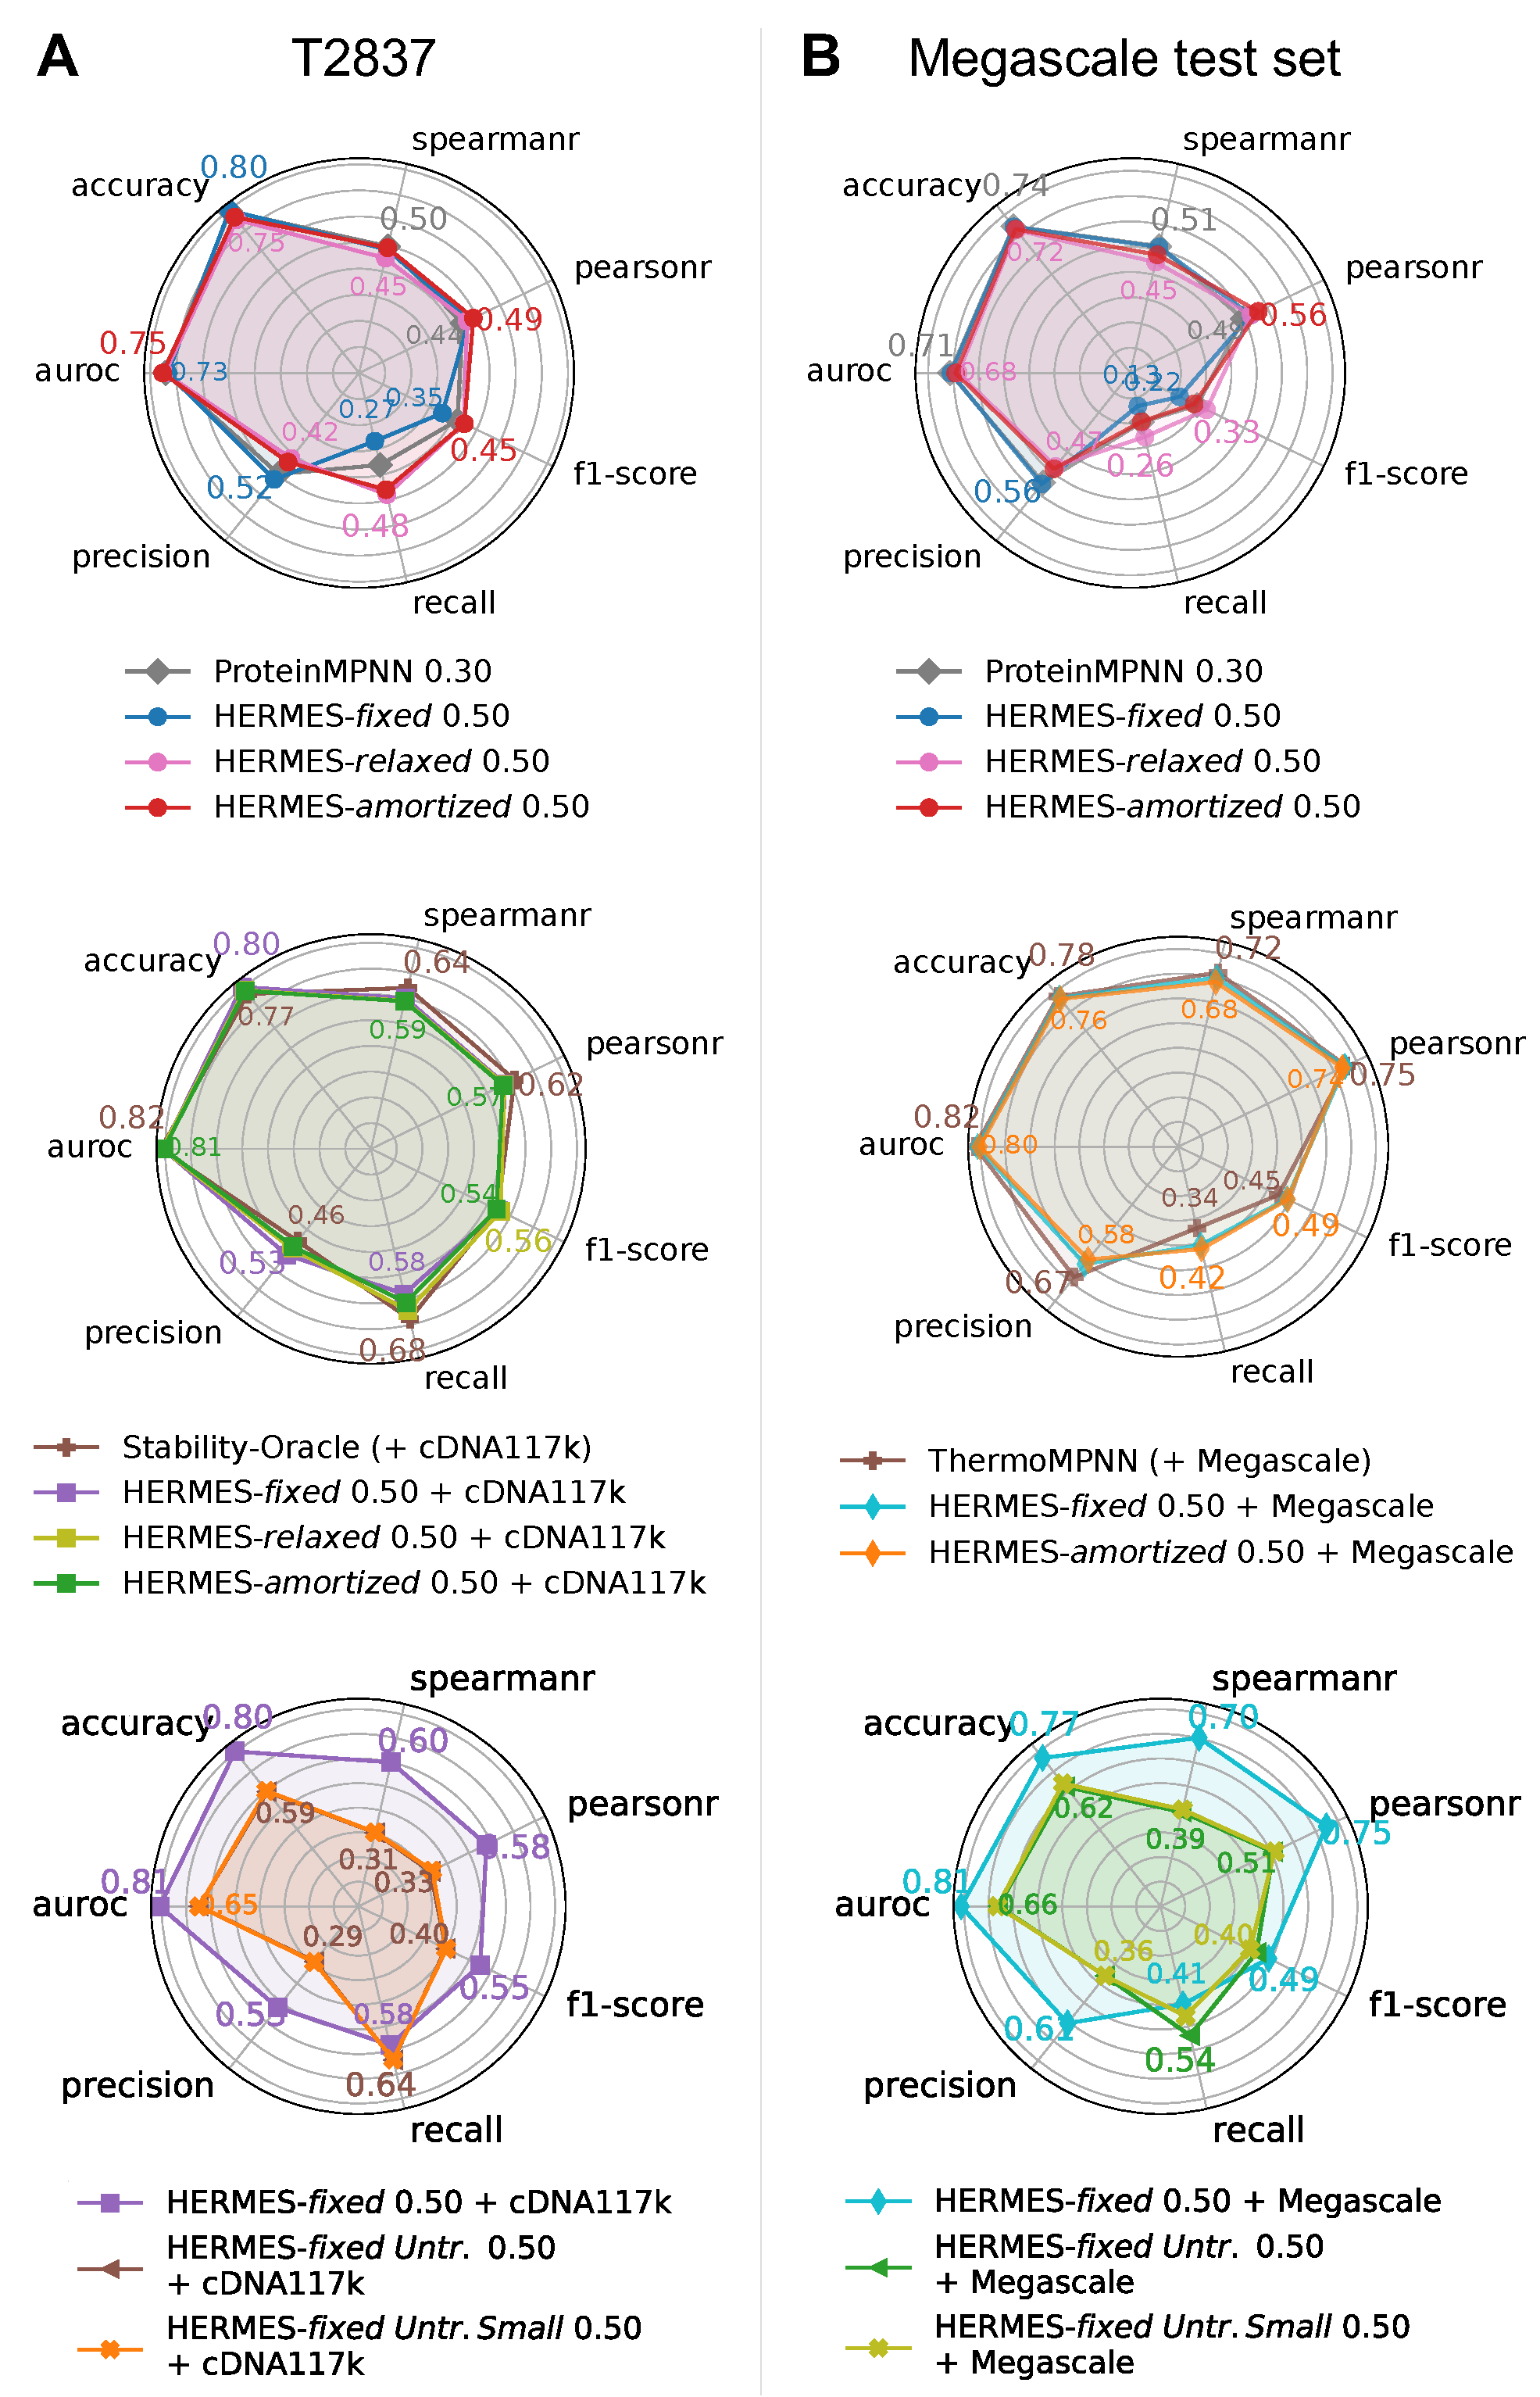
\includegraphics[width=0.70\textwidth]{figures/radial_plots__noise__no_numbers.pdf}
    \figcaption{Predicting mutational effects on thermodynamic folding stability.}{
    Stabilizing-versus-destabilizing classification metrics are computed using $\Delta\Delta G < 0$
    (experimental) and $\Delta \log p > 0$ (predicted) as cutoffs for stabilizing mutations.
    \textbf{(A)} T2837 results: zero-shot models (top) and models fine-tuned or only trained on
    cDNA117k (middle and bottom). \textbf{(B)} Megascale test set results: zero-shot models (top)
    and models fine-tuned or only trained on the Megascale training set (middle and bottom). Model
    names indicate the architecture, the coordinate-noise amplitude used, and when applicable, the
    fine-tuning dataset (listed after ``$+$"); \textit{Untr.} is short for \textit{Untrained},
    indicating models that had no pre-training and were instead only trained on stability effects.
    Only models trained with coordinate noise are shown; the noise amplitude is indicated within
    each model name {as standard deviation in~\AA~units}. Results for models trained without noise
    are provided in Fig.~\ref{fig:radial_plots__no_noise}.
    }
   \label{fig:radial_plots__noise}
\end{figure}

\noindent {\bf Training and test Data.} To enable a direct comparison with recent structure-based
stability predictors, we fine-tuned and evaluated HERMES on the same benchmark splits used by
RaSP~\citep{blaabjerg_rapid_2023}, Stability-Oracle~\citep{diaz_stability_2024}, and
ThermoMPNN~\citep{dieckhaus_transfer_2024}. Specifically, we (i) trained on the RaSP Rosetta-derived
stability dataset and tested on the experimental benchmark used in RaSP, (ii) used
Stability-Oracle's curated cDNA117k training set and T2837 test set; training on 117k $\Delta\Delta
G$ values from ref.~\citep{tsuboyama_mega-scale_2023} filtered by enforcing $\leq 30\%$ sequence
identity to the test set, and (iii) trained on ThermoMPNN's Megascale \textit{train} split and
evaluated on its Megascale \textit{test} split, both from ref.~\citep{tsuboyama_mega-scale_2023};
training on 216k and testing on 28k mutation effects with 25\% sequence-identity cutoff. Because
these splits are defined by the original studies, our results are directly comparable across
methods. We additionally note that the Megascale \textit{train} split is not de-duplicated against
T2837, and six of the T2837 proteins ($\sim 5\%$) have $>90\%$ sequence-similar homologs in the
Megascale training set; see Methods for more details on these training and test sets.\\



\noindent\textbf{Noise and side-chain relaxation improve zero-shot model predictions.} We first
evaluated the \emph{zero-shot} HERMES models (no fine-tuning on experimental data) on the T2837 and
Megascale test sets (Fig.~\ref{fig:radial_plots__noise}, \ref{fig:radial_plots__no_noise}).
Pre-training on structures with Gaussian coordinate noise (0.5~\AA{} s.d.) improves performance,
consistent with prior work~\citep{dauparas_robust_2022, pun_learning_2024}. Relative to
HERMES-\emph{fixed}, the packing-aware HERMES-\emph{relaxed} achieves significantly higher recall
(0.48 vs. 0.27; p-value $<$ 0.01), with only a slight loss in precision, leading to a higher overall
F1-score. HERMES-\emph{amortized} performs similarly to HERMES-\emph{relaxed}: on T2837, and on
Megascale, it shows slightly lower recall and F1 while still outperforming HERMES-\emph{fixed}; the
p-values for the significance of these performance differences are reported in
Fig.~\ref{fig:t2837_and_megascale_pairwise_pvalues_permutation}.

To test whether packing awareness preferentially improves predictions for substitutions that perturb
local packing, we stratified mutations by residue size. Wild-type and mutant residues were assigned
to small, medium, or large classes using normalized van der Waals volumes~\citep{mei_new_2005}, and
we evaluated stabilizing-versus-destabilizing classification performance within each $\wt \to \mt$
size-transition group (Fig.~\ref{fig:megascale_precision_recall_f1_by_size_cutoff_0p0}).


Switching from HERMES-{\em fixed} to HERMES-{\em relaxed} yielded the largest recall gains in
identifying stabilizing substitutions between residues with substantially different sizes. This
improvement was most pronounced for large$\to$small substitutions: HERMES-{\em fixed} is constrained
by the rigid wild-type cavity, preventing it from recognizing that mutations that create voids could
be stabilizing, whereas HERMES-{\em relaxed} can repack neighbors to fill the space and stabilize
the smaller side chain. While precision changes varied across size categories, F1-score improved in
all categories, with the largest gains occurring for small$\to$large substitutions, where relaxation
can reorganize the local environment to accommodate bulkier side chains that would otherwise clash.
Interestingly, HERMES-\emph{amortized}, which learned packing implicitly through fine-tuning, showed
comparable improvements for large$\to$small substitutions but much weaker gains for small$\to$large
substitutions. This could suggest that stabilizing small$\to$large substitutions may be
underrepresented in the fine-tuning training set; the p-values associated with the significance of
performance differences between models within each size-transition category, and within models
across different size-transition categories are reported in
Figs.~\ref{fig:pvalues__bucketed_by_size__between_small_large_buckets__vertical},~\ref{fig:t2837_and_megascale_pairwise_pvalues_permutation}.

For comparison, we evaluated ProteinMPNN~\citep{dauparas_robust_2022}
on the same tasks. ProteinMPNN outperformed HERMES-{\em fixed}, and performed on par with
HERMES-\emph{relaxed} on both small$\to$large and large$\to$small mutations
(Fig.~\ref{fig:megascale_precision_recall_f1_by_size_cutoff_0p0},~\ref{fig:pairwise_pvalues_permutation_bucketed_by_sizereduced_precision_recall_f1}).
We attribute this performance to ProteinMPNN's input representation: by conditioning only on
backbone coordinates and residue identities, ProteinMPNN is less constrained by the explicit
wild-type side-chain geometry compared to the all-atom HERMES-{\em fixed} model. This architectural
choice enables implicit reasoning about side-chain flexibility, achieving results comparable to
using explicit relaxations in HERMES-{\em relaxed}. Notably, ProteinMPNN performed better than
HERMES-{\em amortized} on small$\to$large substitutions.\\



\begin{figure}
    \centering
    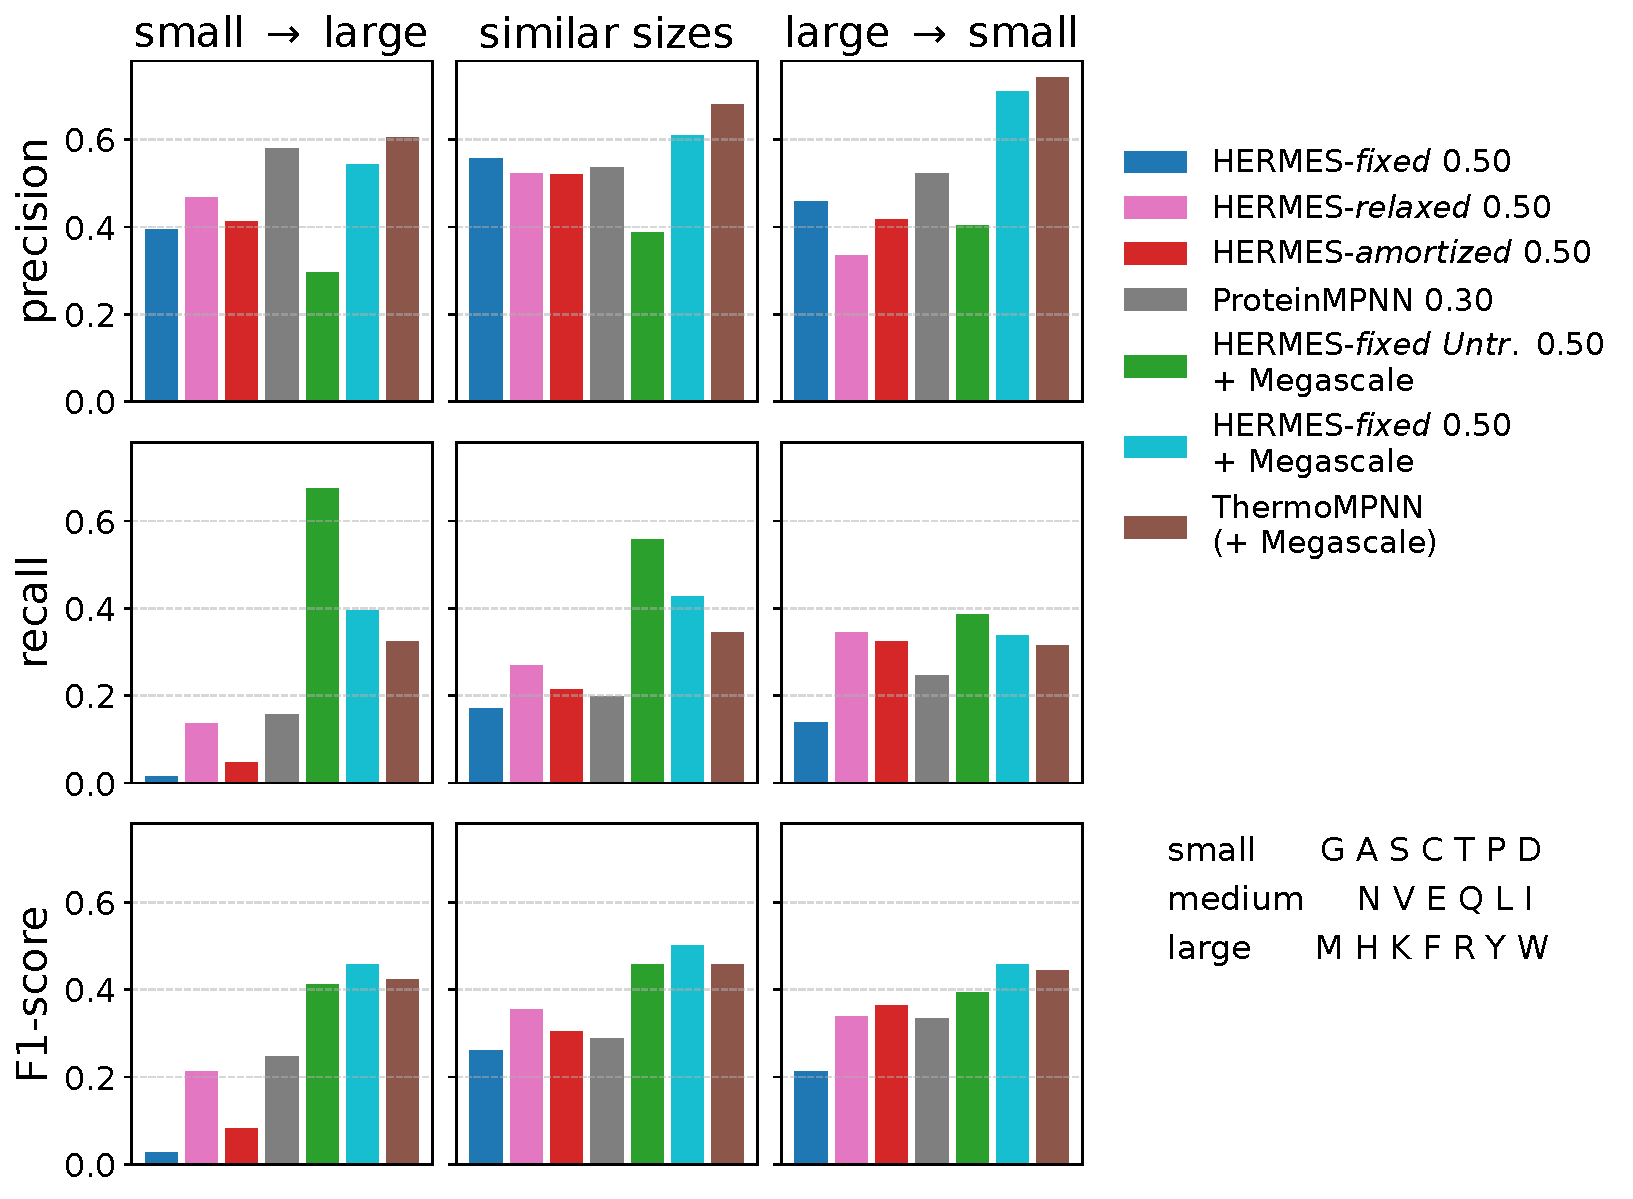
\includegraphics[width=0.9\textwidth]{figures/barplots_bucketed_by_size__zeroshot_plus_finetuned__precision_and_recall_and_f1.pdf}
    \figcaption{Impact of amino acid size changes on predicting mutational effects on protein
    stability.}{
    Amino acids are grouped into three size classes based on van der Waals volume (as listed), and
    predictions are stratified by wild-type and mutant size classes; ``similar sizes" denote
    substitutions within the same class.
    Stabilizing-versus-destabilizing classification metrics (rows) are then computed and shown for
    each stratum (columns), using $\Delta\Delta G < 0$ (experimental) and $\Delta \log p > 0$
    (predicted) as cutoffs for stabilizing mutations.
    P-values for pairwise model comparisons are shown in
    Fig.~\ref{fig:pairwise_pvalues_permutation_bucketed_by_sizereduced_precision_recall_f1}, and
    p-values comparing each model's performance on small$\to$large vs. large$\to$small substitutions
    are shown in Fig.~\ref{fig:pvalues__bucketed_by_size__between_small_large_buckets__vertical}.
    Model names indicate the architecture, the coordinate-noise amplitude used during pre-training
    {as standard deviation in~\AA~units}, and when applicable, the fine-tuning dataset (listed after
    ``$+$").
}    \label{fig:megascale_precision_recall_f1_by_size_cutoff_0p0}
\end{figure}
\noindent {\bf Fine-tuned HERMES models achieve state-of-the-art performance for stability effect
prediction.}
When fine-tuning on the respective stability effect datasets, HERMES outperformed RaSP
(Fig.~\ref{fig:rasp_exp}), and matched the performance of Stability-Oracle
(Fig.~\ref{fig:radial_plots__noise}A,~\ref{fig:t2837_broken_down_and_comparison}) and ThermoMPNN
(Fig.~\ref{fig:radial_plots__noise}B).
These results underscore both the effectiveness of the HERMES architecture and the importance of
fine-tuning data for test-time accuracy. HERMES was also robust to using ESMFold-resolved
structures~\citep{lin_evolutionary-scale_2023} for either fine-tuning or inference
(Fig.~\ref{fig:radial_plots__esmfold}), supporting practical use cases where only computationally
predicted structures are available.

Removing pre-training on wild-type amino-acid classification significantly degraded performance:
HERMES models trained {\em only} for stability prediction performed poorly when trained on either
cDNA117k or Megascale, even after reducing capacity from 3.5M parameters to 50k to mitigate
overfitting (Fig.~\ref{fig:radial_plots__no_noise}). A similar failure mode was reported for
ThermoMPNN on the Megascale training data~\citep{dieckhaus_transfer_2024}.

Finally, fine-tuning on stability effects largely eliminated size-dependent bias, yielding
comparable recall and F1 scores for small$\to$large and large$\to$small substitutions
(Figs.~\ref{fig:megascale_precision_recall_f1_by_size_cutoff_0p0},~\ref{fig:pvalues__bucketed_by_size__between_small_large_buckets__vertical}).\\


\begin{figure}
    \centering
    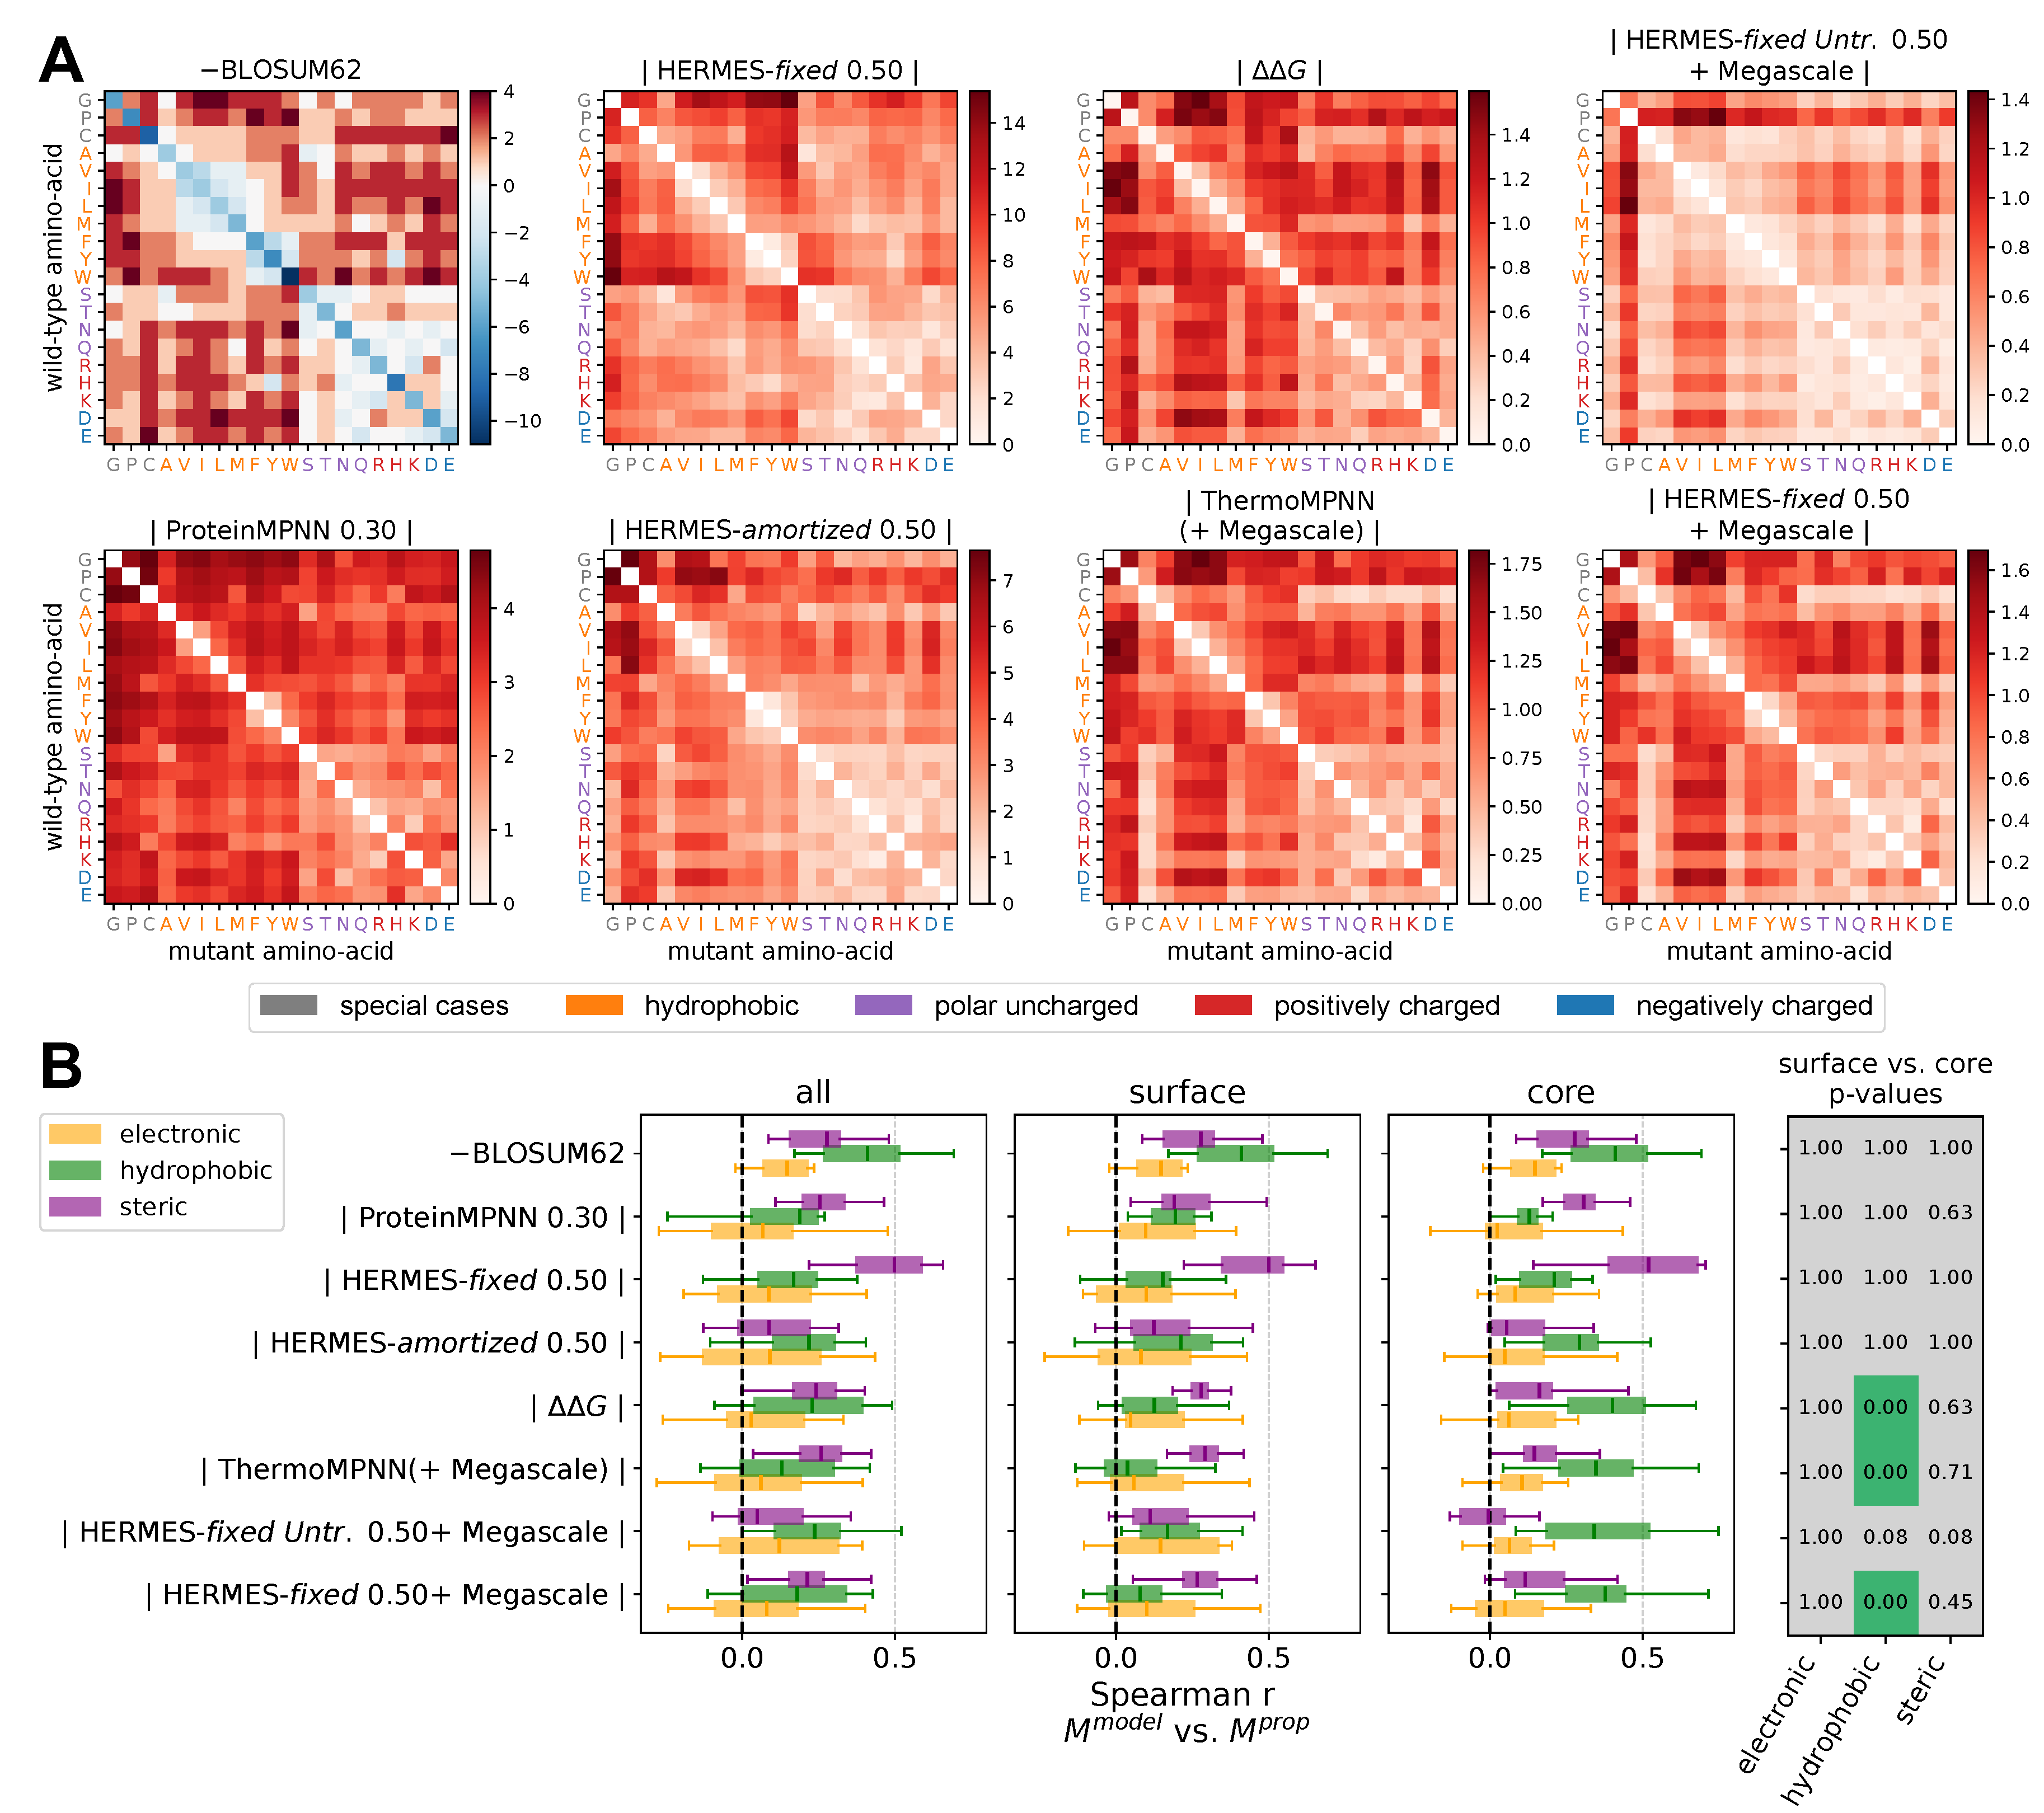
\includegraphics[width=1.0\textwidth]{figures/confusion_matrices_and_boxplot_with_abs.pdf}
    \figcaption{Uncovering mutation preferences via model-averaged substitution matrices.}{
    \textbf{(A)} 
    Heatmaps of model-averaged substitution matrices $M^{\model}$ computed by averaging over the
    Megascale test set, shown alongside BLOSUM62 and and the experimental matrix of mean
    $|\Delta\Delta G|$ values across mutations.
    Spearman correlations between matrices are reported in
    Fig.~\ref{fig:spearmanr_between_model_average_substitution_matrices}. Core- and
    surface-restricted matrices (core: SASA $< 1 \AA^2$; surface: SASA $> 3 \AA^2$) are shown in
    Fig.~\ref{fig:average_prediction_matrices__abs_symm__part_1}~and~\ref{fig:average_prediction_matrices__abs_symm__part_2}.
    \textbf{(B)} For each model and site subset (all, surface, core), boxplots summarize Spearman
    correlations between $M^{\model}$ and property-difference matrices $M^{\prop}$, grouped by
    property class (color). P-values from two-tailed t-tests comparing the surface vs. core
    correlations within each property class are shown on the right. P-values for between-model
    comparisons of property-class correlations are shown in
    Fig.~\ref{fig:correlation_to_aa_properties__significance}.
      }
    \label{fig:correlations_to_aa_properties}
\end{figure}

\noindent \textbf{Biophysical interpretation of HERMES predictions for mutational stability
effects.}
We sought to quantify how much models' mutation preferences could be explained by amino-acid
physicochemical properties. Specifically, we asked which properties are shared by amino-acid pairs
that the model treats as interchangeable, i.e., substitutions with $\Delta \hat{F} \approx 0$ on
average.

To do this, we constructed model-averaged substitution matrices $M^{\model}$ whose $(\alpha,\beta)$
entry represents how neutrally the model treats exchanging amino acids $\alpha$ and $\beta$. For
each pair $(\alpha,\beta)$, we computed the model-predicted mean {\em absolute} effect,
$M^{\model}_{\alpha, \beta} = \langle |\Delta \hat{F}^{(\model)}_{\alpha,\beta} |\rangle$, where
$\langle \cdot \rangle$
denotes averages over all $\alpha\to \beta$ and $\beta\to \alpha$ substitutions in the Megascale
test set. This procedure yields a symmetric, non-negative $20\times 20$ matrix for each model, in
which values approaching zero indicate greater predicted interchangeability. For comparison, we
constructed an analogous matrix using experimentally measured $|\Delta\Delta G|$ values from the
Megascale test set ($M^{|\Delta\Delta G|}$), and include the BLOSUM62 substitution matrix as an
additional reference.

Following ref.~\cite{pyo_data-driven_2025}, we also constructed symmetric, nonnegative matrices of
\emph{absolute amino-acid property differences}. Specifically, we considered 50 quantitative
properties spanning (i) hydrophobic, (ii) electronic, and (iii) steric categories
(Table~\ref{table:aa_properties}), yielding 50 property-specific matrices $M^{\prop}$ with the
$(\alpha,\beta)$ entry: $M^{\prop}_{\alpha,\beta} = |\prop_\alpha - \prop_\beta|$. Smaller values
indicate greater similarity between the two amino acids with respect to the specified property.


To quantify which biophysical properties each model tends to preserve, we computed the Spearman
correlation between the model-averaged substitution matrix
 $M^{\model}$ and each of property-specific amino acid distance matrix $M^{\prop}$
 (Fig.~\ref{fig:correlations_to_aa_properties}B).
Consistent with the size-stratified analysis
(Fig.~\ref{fig:megascale_precision_recall_f1_by_size_cutoff_0p0}), HERMES-{\em fixed} predicted
amino-acid interchangeability align most strongly with steric properties, particularly average
buried-residue volume (Spearman $r =0.66$) and normalized van der Waals volume (Spearman $r =
0.64$). This correlations was significantly stronger than for the other models (p-values in
Fig.~\ref{fig:correlation_to_aa_properties__significance}).
In contrast, BLOSUM62, derived from evolutionary substitution frequencies, preferentially preserves
hydrophobic properties. When restricting $M^{\model}$ to core residues (SASA $< 1$\AA$^2$), the
interchangeability matrix associated with stability-fine tuned models {(e.g.
$M^{\text{HERMES-\textit{fixed} 0.50 + Megascale}}$)} showed stronger alignment with hydrophobic
properties, to levels comparable to BLOSUM62 and consistent with the experimental matrix
$M^{|\Delta\Delta G|}$.
Zero-shot models instead did not show a comparable increase in hydrophobic preservation when
restricting to the core (Fig.~\ref{fig:correlations_to_aa_properties}B).\\




\begin{figure}[ht!]
    \centering
    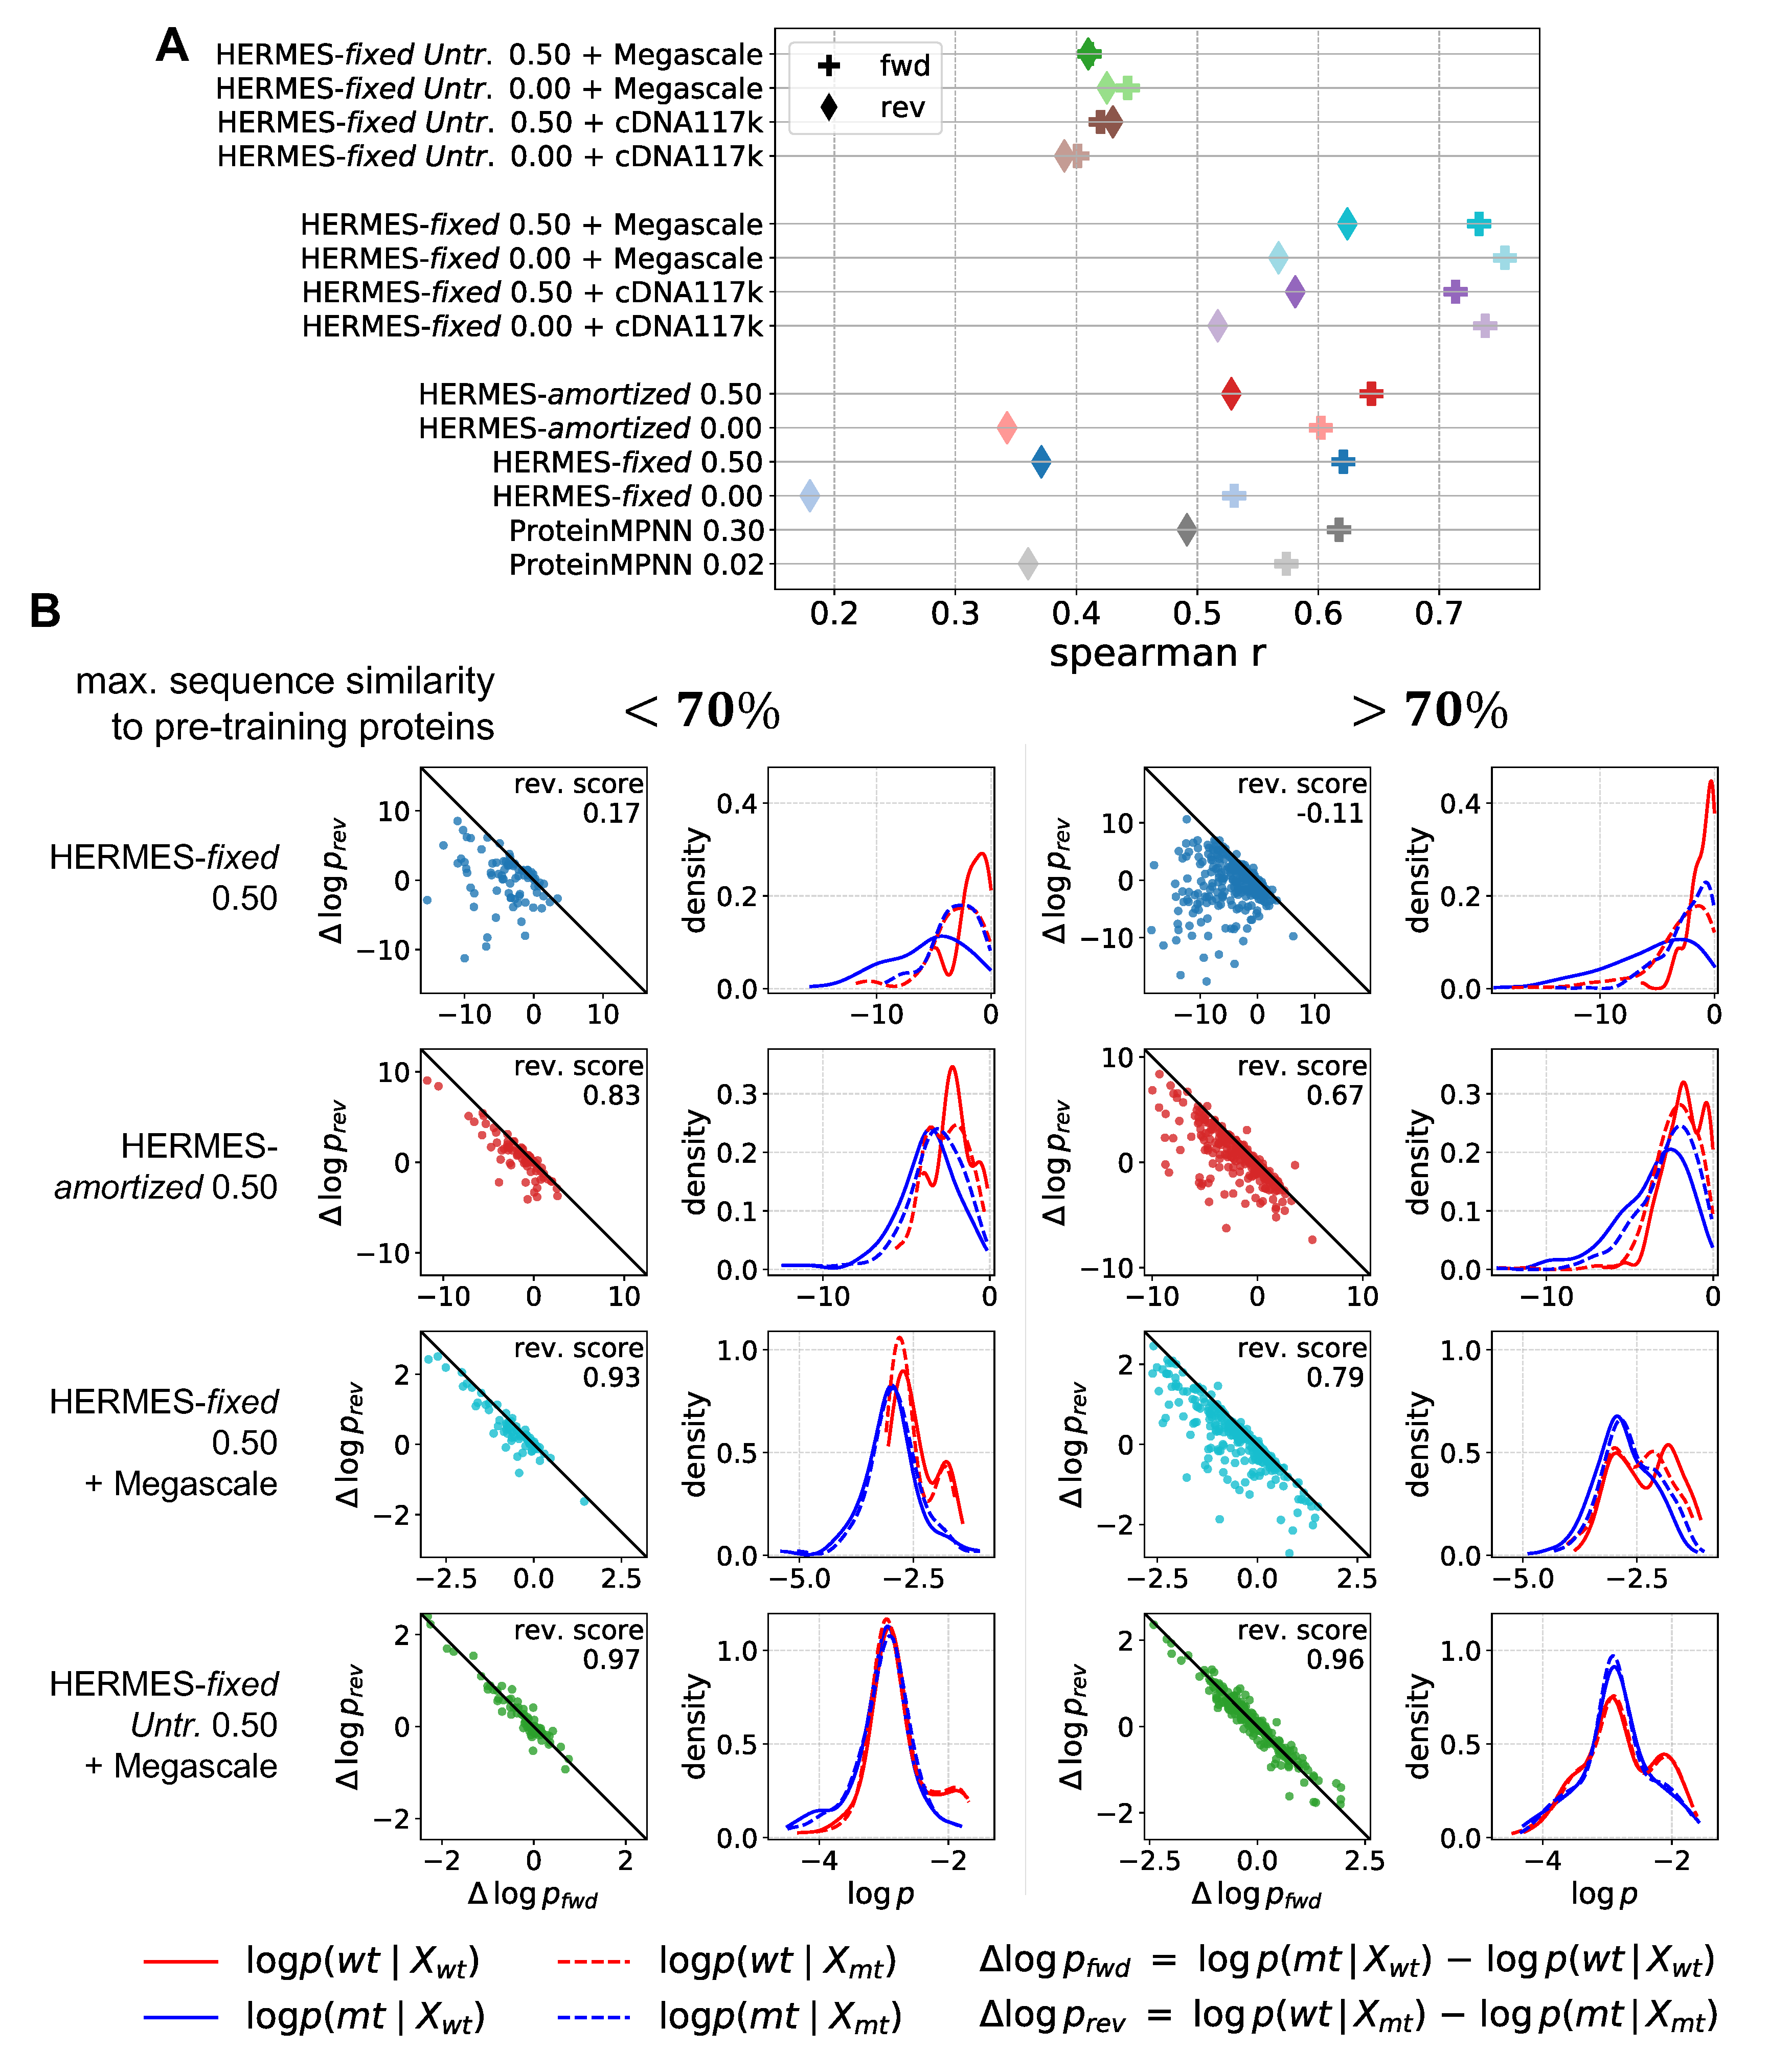
\includegraphics[width=0.9\textwidth]{figures/reversibility_and_wt_bias.pdf}
    \figcaption{Identifying model biases with structure-conditioned reversibility}{
    \textbf{(A)} 
   Spearman correlations between experimental stability changes ($\Delta\Delta G$ and model
   predictions on the Ssym dataset are shown. For each model, we report correlations for forward
   substitutions ($\Delta \log p_{fwd}$ vs. $\Delta\Delta G$) and the reverse substitutions ($\Delta
   \log p_{rev}$ vs. $-\Delta\Delta G$). {\bf(B)} Ssym proteins are stratified by their maximum
   sequence identity to pre-training proteins ($\geq 70\%$ vs. $< 70\%$). For each split (columns)
   and four representative HERMES variants (rows), the left panel shows the scatter plots for
   $\Delta \log p_{fwd}$ vs. $\Delta \log p_{rev}$; an unbiased model should exhibit strong
   anti-correlation, summarized by the reversibility score (rev.; higher is more reversible;
   Eq.~\ref{eq:rev_score}). Reversibility is highest for the model not pre-trained on wild-type
   amino-acid classification (green; bottom row) and is consistently higher for the low-similarity
   subset. Fig.~\ref{fig:ssym_antisymmetry_reversibility_score_results} shows the reversibility
   scores across all models in (A). In each column, the right panel shows the distributions of the
   log-probabilities that make up $\Delta \log\,p_{fwd} = \log p (\mt | X_\wt) - \log p (\wt|X_\wt)$
   (solid lines) and $\Delta \log\,p_{rev} = \log p (\wt | X_\mt) - \log p (\mt|X_\wt)$ (dashed
   lines). All models except for the one that was \textit{not} pre-trained on wild-type amino-acid
   classification (last row) exhibit elevated $\log p(\wt\,|X_{\wt})$.
    }
    \label{fig:ssym_figure}
\end{figure}
   
\noindent{\bf Reversibility and path-independence of HERMES predictions with respect to mutations.}
Mutational effects are, in principle, reversible: the effect of substituting a residue from amino
acid $\alpha$ to $\beta$ should be equal in magnitude and opposite in sign to the reverse change,
i.e., $\Delta F_{\alpha \to \beta} = -\Delta F_{\beta\to \alpha}$. Moreover, equilibrium quantities
such as protein stability free energy are state functions. As such, the net effect of a multi-step
substitution depends only on the initial and final amino acids, not on the mutational path. For a
path $\alpha \to \beta \to \gamma$, this implies: $\Delta F_{\alpha\to \gamma} = \Delta F_{\alpha\to
\beta} + \Delta F_{\beta\to \gamma}$.



HERMES predicts mutation effects as differences in amino-acid-specific log-probabilities (logits)
$\log p(aa | X_{aa})$ (both zero-shot and after fine-tuning). As log-probability differences under a
fixed structural context, these predictions satisfy reversibility by construction:
\EQ 
\Delta \hat F^{(\text{model})}_{\alpha\to \beta} = \log P(\beta | X_{\beta}) - \log P(\alpha
|X_{\alpha}) = -\Delta \hat F^{(\text{model})}_{\beta\to \alpha}
\label{eq:reversibility}
\EE
where we set $X_{\alpha}= X_{\beta}$ for HERMES-{\em fixed} and HERMES-{\em amortized}, and
$X_{\beta}= \hat X_{\alpha\to \beta}$ for HERMES-{\em relaxed}. Path-independence follows similarly.
In contrast, other structural models such as Stability-Oracle~\citep{diaz_stability_2024} require
explicit $19\times$ data augmentation (termed ``thermodynamic permutation augmentation" in
ref.~\citep{diaz_stability_2024}) to enforce these properties.

Alternatively, reversibility can be assessed in a structure-conditioned
manner~\citep{blaabjerg_rapid_2023, dieckhaus_transfer_2024}, where the effects of forward
$\alpha\to \beta$ and reverse $\beta \to \alpha$ substitutions are computed using the outgoing
structural contexts, i.e., $\alpha\to \beta$ is conditioned on $X_{\alpha}$ and $\beta\to\alpha$ on
$X_{\beta}$ (Extended Methods, Appendix~\ref{sec:hermes_appendix}). Under this transformation, we do
not automatically expect a
``structure-conditioned reversibility", as forward and reverse transitions are conditioned on
different structures. However, a well-balanced model should have near-reversibility in this setting,
making this a stringent test of model bias. We measured structure-conditioned reversibility on the
Ssym dataset, which contains wild-type and single-mutant structures for 352 mutations across 19
proteins~\citep{pancotti_predicting_2022}.
For each mutation, we computed a ``forward" effect ($\wt \to\mt$, conditioned on the wild-type
structure) and a ``reverse" effect ($\mt \to\wt$, conditioned on the mutant structure).


We found that zero-shot HERMES models and ProteinMPNN predict stability effects more accurately for
forward substitutions ($\wt \to\mt$) than for the reverse direction, consistent with previous
observations~\citep{blaabjerg_rapid_2023, dieckhaus_transfer_2024} (Fig.~\ref{fig:ssym_figure}A).
Adding coordinate noise during pre-training and fine-tuning on stability effects both reduced this
forward-reverse disparity, but did not eliminate it. Models trained {\em only} on stability effects
showed little or no disparity, albeit with substantially lower overall accuracy.
Across all pre-trained models, the predicted stability effects of forward mutations from the
wild-type tend to have larger magnitudes than those of the corresponding reverse mutations
(Fig.~\ref{fig:ssym_figure}B, scatterplots). This bias stems from the elevated log-probabilities
assigned to wild-type amino acids in wild-type structure neighborhoods $\log p(\wt | X_{\wt})$
(Fig.~\ref{fig:ssym_figure}B, density plots), suggesting a wild-type preference that may reflect
pre-training memorization. Consistently, stratifying Ssym proteins by sequence similarity to the
pre-training set (Extended Methods, Appendix~\ref{sec:hermes_appendix}) yielded a modest reduction
in wild-type preference for lower-similarity
proteins (Fig.~\ref{fig:ssym_figure}B). A more detailed characterization of this bias is left to
future work.

\begin{figure}[t!]
    \centering
    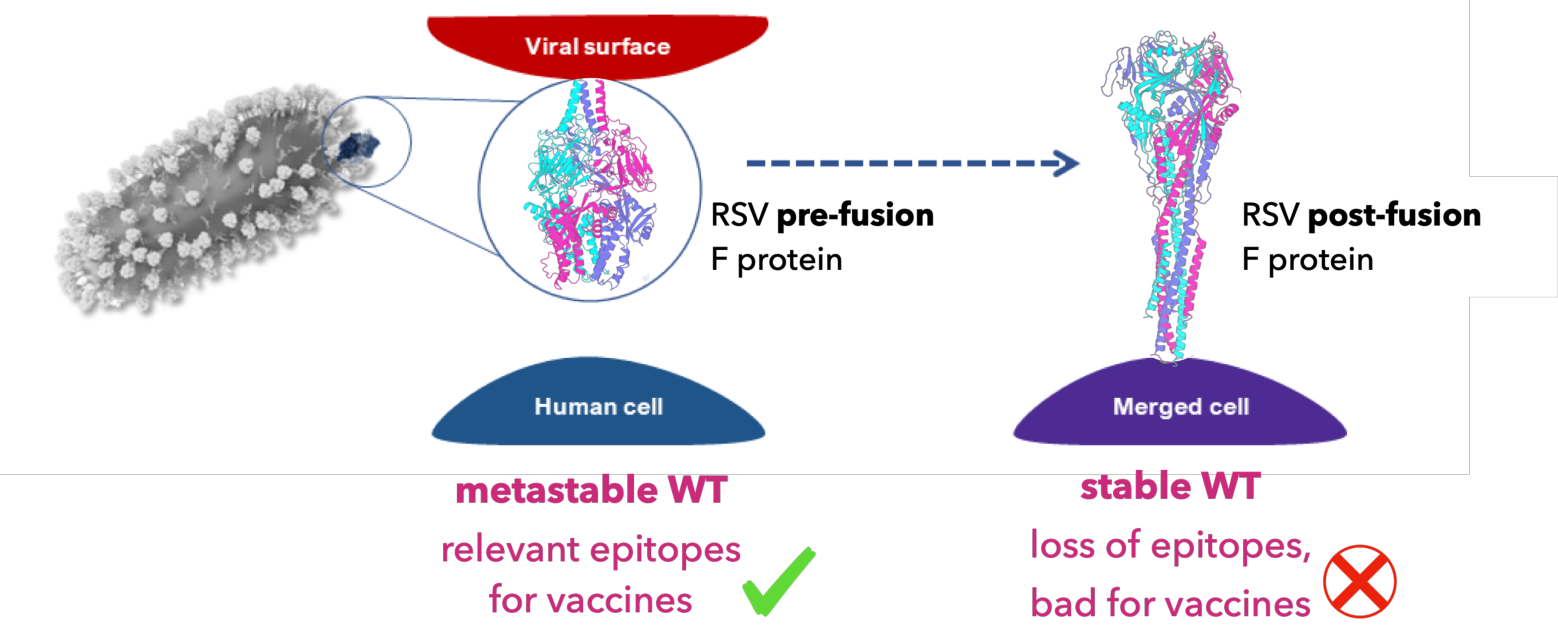
\includegraphics[width=0.9\linewidth]{figures/antigen_design_concept.pdf}
    \figcaption{\GM{Overview of structure-based vaccine design against enveloped viruses.}}{
        \GM{
            A large proportion of viruses are enveloped by a bi-lipid membrane akin to that of human cells,
            The infect human cells, they make use of specialized proteins that latch onto the cell's
            membrane and ``fuse" it to the virus' envelope. This fusion process is enabled by a
            conformational change in the fusion protein: from a ``pre-fusion" to a ``post-fusion"
            conformation.
            Naturally, vaccines should be engineered to elicit immune responses that target epitopes
            presented \textit{before} the virus has infected the cell, i.e. while the fusion protein
            is in the pre-fusion conformation.
            However, the wild-type of fusion viruses is generally more stable in the post-fusion
            conformation.
            Therefore, the field of structure-based vaccine design has proposed to use vaccines
            containing engineered mutants of the fusion proteins that are more stable in
            pre-fusion relative to post-fusion.
            Figure adapted from \url{https://www.niaid.nih.gov/diseases-conditions/safe-and-effective-rsv-protein-vaccines}.
        }
    }
    \label{fig:antigen_design_concept}
\end{figure}


\subsection{Antigen stabilization with HERMES for vaccine design}
Structure-based vaccine design seeks to increase vaccine efficacy by \GM{engineering viral envelope
glycoproteins (hereafter, ``antigens") to be more stable in their pre-fusion conformation,
relative to their post-fusion conformation (Figure~\ref{fig:antigen_design_concept}).
Pre-fusion stabilization} enriches presentation of neutralization-relevant epitopes and can bias elicited immune responses
toward protective specificities.
\GM{In the literature, it is achieved by applying a minimal set of mutations to the fusion protein that either improve the stability
of the pre-fusion conformation, or decrease that of the post-fusion conformation, while preserving the relevant
epitopes~\citep{mclellan_structure-based_2013, gonzalez_general_2024, bakkers_efficacious_2024, milder_universal_2022, phan_conserved_2022}.

Practitioners often classify mutations in different types
based on the manner in which they provide relative pre-fusion stabilization (hereafter, ``antigen stabilization").
For example, {\em Cavity-filling mutations} mutations stabilize the pre-fusion conformation by filling cavities
located within the hydrophobic core, by inserting a larger hydrophobic side-chain.
{\em Proline mutations} instead are often used to impede post-fusion $\alpha$-helix formation and
stabilize pre-fusion conformations, due to proline's unique lack of amide hydrogens which prevents
it from taking part in stable $\alpha$-helices.
Other mutation types include {\em electrostatic mutations}, which introduce polar or charged amino acids in environments
where they can engage in stabilizing electrostatic interactions,
and finally {\em synergistic mutations}, which involve applying multiple mutations so that they positively interact
through a variety of mechanisms.
We show examples of mutation types in Fig.~\ref{fig:antigen_figure_of_different_types_of_mutations}A.
}

\GM{
The use of computational tools to guide antigen stabilization has precedents in the literature,
but it is largely limited to the use of scoring functions like Rosetta~\citep{gonzalez_general_2024, phan_conserved_2022},
with few closed-source attempts to use machine learning~\citep{bakkers_efficacious_2024}.
Therefore, we sought out to test whether HERMES can be used to aid vaccine design campaigns.

Unfortunately, large scale datasets of experimentally-validated mutations are not yet present.
Thus, we started the campaign by manually collecting 33 previously reported antigen-stabilizing mutations drawn from
five viral antigens: Influenza HA~\citep{milder_universal_2022} (3 mutations),
RSV-F~\citep{mclellan_structure-based_2013, lee_rational_2024} (7 mutations),
hMPV-F~\citep{gonzalez_general_2024, bakkers_efficacious_2024, phan_conserved_2022} (11 mutations),
DENV-E~\citep{phan_conserved_2022} (8 mutations), and SARS-CoV-2 spike
protein~\citep{hsieh_structure-based_2020} (4 mutations).
We then benchmarked model performance on their ability to identify the specific mutants
as the most pre-fusion-stabilizing within their respective sites; essentially evaluating per-site recall.
We scored mutations using zero-shot and
stability-fine-tuned variants of ProteinMPNN and HERMES. Importantly, none of the stabilized
variants in this benchmark appeared in the training data of any HERMES model, either during
pre-training or during stability fine-tuning.
}

\begin{figure}[t!]
    \centering
    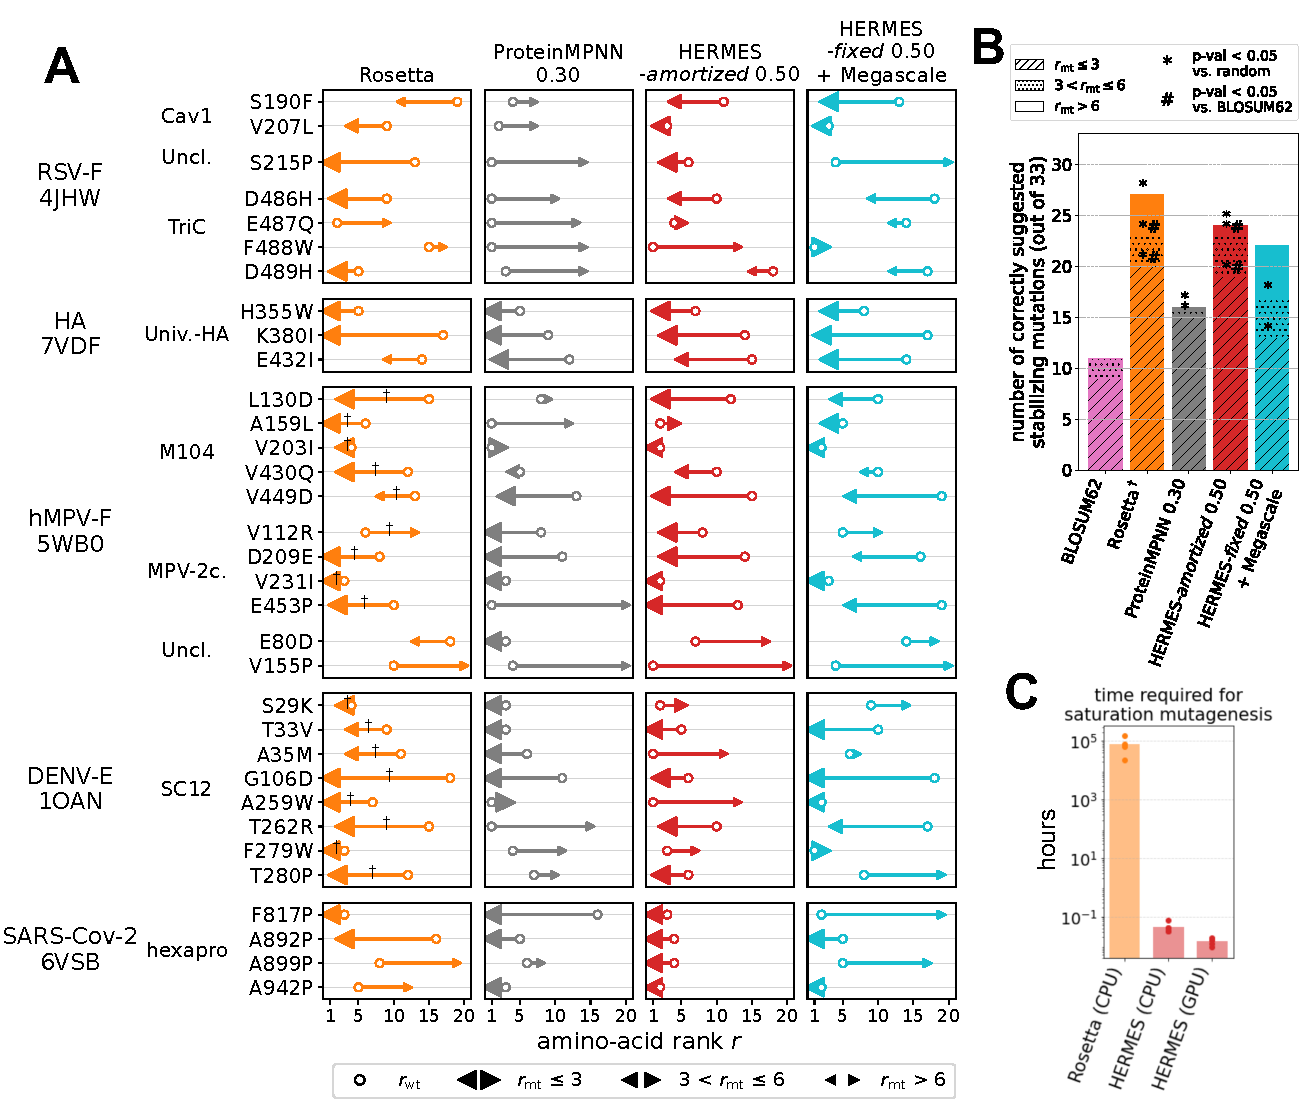
\includegraphics[width=1.0\linewidth]{figures/antigen_figure_main_results_with_time.pdf}
    \figcaption{Recovering previously-identified antigen-stabilizing mutations with HERMES.}{
    \textbf{(A)} Model recall is evaluated on 33 previously reported antigen-stabilizing mutations
    (rows) across five viral antigens. For each antigen, the PDB structure used for scoring is
    indicated. Mutations are specified as wild-type$\to$mutant substitutions at the annotated site.
    Four models (columns) are compared, as labeled above each column; see
    Table~\ref{table:antigen_results} for a more extensive comparison of models on this task. Arrows
    depict the change in predicted rank from the wild type (open circle) to the stabilizing mutant
    (arrow tip); arrow size indicates whether the mutant ranks in the top 3 (large), ranks 4--6
    (medium), or ranks $>6$ (small). The $\dagger$ symbols mark mutations originally proposed as
    stabilizing by Rosetta. ``Univ.-HA" stands for ``Universal-HA"; ``MPV-2c." stands for
    MPV-2cREKR; ``Uncl." stands for ``Uncleaved Prefusion-Closed".
    {\bf (B)} Counts of correctly
    prioritized antigen-stabilizing mutations ($r_\mt < r_\wt$), stratified by predicted rank group:
    strongly suggested ($r_\mt \leq 3$), moderately suggested ($3 < r_\mt \leq 6$), or weakly
    suggested ($6\leq r_\mt$) are shown for each model. For comparison, BLOSUM62 is used to rank
    substitutions into the ($r_\mt \leq 3$) or ($3 < r_\mt \leq 6$) groups; under this scheme the
    wild-type residue is always ranked first. Statistical enrichment is assessed by comparing the
    number of strong/moderate recalls to a random-ranking baseline and to BLOSUM62 (denoted by ($*$)
    and ($\#$), respectively, when binomial tests corrected p-value$<0.05$; see Methods).
    We note that all structures were considered in their native multimeric state, generating
    symmetric partners with PyMOL when necessary.
    \GM{{\bf (C)} Estimated times for saturation mutagenesis predictions on the viral antigens considered
    in this study. Each dot is an antigen. Times shown are for a single CPU and a single NVIDIA A40 GPU.
    See Table~\ref{table:speed_on_antigens} for precise per-antigen times.}
    }
    \label{fig:antigen_figure_main_results}
\end{figure}
 
To quantify performance, we emulated a simple model-guided selection workflow in which a
practitioner considers substitutions at a site in descending order of model scores. For each known
stabilizing mutation, we record its rank $r_\mt$ among all 20 amino acids at that position and
compare it to the wild-type rank $r_\wt$. We posit that a practitioner would select a particular
mutant for experimental validation if (1) its rank $r_\mt$ is better (lower) than that of the
wild-type $r_\wt$, and (2) its rank is among the top-scoring candidates (lower end). We categorize
each predicted-stabilizing mutation (i.e., with $r_\mt < r_\wt$) as strongly suggested ($r_\mt \leq
3$), moderately suggested ($3 < r_\mt \leq 6$), or weakly suggested ($r_\mt > 6$)
(Fig.~\ref{fig:antigen_figure_main_results} {and Table~\ref{table:antigen_results}}). This scheme
would group mutations with similar physico-chemical properties into the same rank class.
Consequently, models are generally not penalized for ranking a biophysically similar alternative
above a known stabilizing mutant, making our performance metrics robust to fine-grained rank
differences in different models (see Fig.~\ref{fig:antigen_heatmap} and Appendix~\ref{sec:hermes_appendix}
for a more detail discussion on antigen-stabilizing mutations).

Figs.~\ref{fig:antigen_figure_main_results},~\ref{fig:antigen_figure_of_different_types_of_mutations}
{and Table~\ref{table:antigen_results}} summarize predictions across the 33 stabilizing mutations we
studied. Among the machine-learning methods, HERMES-\emph{amortized} performs best: it assigns a
better (lower) rank than wild-type to 24 stabilizing mutations, including 19 classified as strongly
suggested ($r_\mt \leq 3$). Notably, stability fine-tuning does not consistently improve performance
over the corresponding zero-shot ProteinMPNN and HERMES-{\em amortized} on this task
(Table~\ref{table:antigen_results}).

For comparison, we also scored each mutant with Rosetta~\citep{chaudhury_pyrosetta_2010},
(Extended Methods, Appendix~\ref{sec:hermes_appendix}).
Rosetta recovers stabilizing mutations on par with HERMES-\emph{amortized}
({Fig.~\ref{fig:antigen_figure_main_results} and} Table~\ref{table:antigen_results}); however, 17
variants in this benchmark were originally selected (by the references that discovered the variants)
using Rosetta-based screening, which partially biases this baseline in Rosetta's favor.
Most importantly, however,
Rosetta inference is substantially more computationally intensive than the machine learning models,
limiting its practicality for predicting the stability effects in high-throughput saturation
mutagenesis \GM{(Fig.~\ref{fig:antigen_figure_main_results}C)}.

To assess statistical enrichment of model predictions over chance, we compared the predicted number
of stabilizing mutations in the strong/moderate categories to a random-ranking baseline using a
binomial test (Extended Methods, Appendix~\ref{sec:hermes_appendix}); p-values are reported in
Fig.~\ref{fig:antigen_pvalues_vs_random}. All models except for HERMES-{\em fixed} and ThermoMPNN
significantly outperform random ranking in
recovering stabilizing mutations with strong or moderate confidence
({Table~\ref{table:antigen_results}}).
As an additional baseline, we tested whether the BLOSUM62 (B62) substitution matrix can prioritize
stabilizing mutations. BLOSUM62 recovers significantly fewer stabilizing mutations in the
strong/moderate categories than HERMES-\emph{amortized} (defined as $r_\mt^{B62} \leq 3$ and
$r_\mt^{B62} \leq 6$, noting that $r_\wt^{B62} = 1$ always; {results shown in
Fig.~\ref{fig:antigen_figure_main_results},} and binomial test p-values reported in
Fig.~\ref{fig:antigen_pvalues_vs_blosum62}), underscoring the value of incorporating structural
context when predicting stabilizing substitutions.

\GM{For a more detailed analysis, we manually annotated the 33 antigen-stabilizing mutations based on their mutation types
(Table~\ref{table:mutation_types}) and accordingly stratified model performance (Fig.~\ref{fig:antigen_figure_of_different_types_of_mutations}B).}
Among the models tested, HERMES-\emph{amortized} most reliably recovers stabilizing proline
mutations (7 out of 8; Fig.~\ref{fig:antigen_figure_of_different_types_of_mutations}B), highlighting
its potential utility for proposing pre-fusion stabilizing prolines. More broadly, all models
recover proline and electrostatic mutations at higher rates than expected under BLOSUM62, whereas
cavity-filling mutations show weaker gains. A plausible explanation is that cavity-filling changes
typically replace a smaller hydrophobic residue with a larger one that preserves core
hydrophobicity. Because such substitutions are common in natural sequence variation, they are partly
captured by a sequence-derived matrix like BLOSUM62. In contrast, proline and charged substitutions
are strongly context-dependent, with effects that hinge on local geometry and environment, and
therefore benefit more from structure-aware modeling; see Appendix~\ref{sec:hermes_appendix} for a more detailed discussion.

Lastly, the synergistic RSV-F TriC mutations are difficult to recover for almost all methods
(Fig.~\ref{fig:antigen_figure_main_results}). This is expected for the three ``acid patch
neutralization" substitutions D486H, D489H, and E487Q~\citep{mclellan_structure-based_2013}, which
were experimentally stabilizing only in combination (i.e., synergy) with
F488W~\citep{mclellan_structure-based_2013}. These four residues are tightly clustered in both
intra- and inter-chain space, consistent with a synergistic (epistatic) mechanism in which the
substitutions act synergistically to stabilize the trimer. A second example of synergy is the DENV-E
pair A259W and T262R, which together introduce a favorable cation-$\pi$ interaction
(Fig.~\ref{fig:antigen_figure_of_different_types_of_mutations}A.4). Because our evaluation scheme
scores mutations in a site-independent manner, the models are not able to capture such multi-residue
dependencies. Specifically, HERMES scores mutations at a single site under the assumption that all
other amino-acid identities remain fixed, and therefore, cannot recover stabilization mechanisms
that arise only from specific combinations of mutations. ProteinMPNN, ThermoMPNN, and Rosetta are
likewise evaluated here under the same site-independent protocol for a fair comparison, although
they can in principle be applied to score multi-residue variants jointly; see Appendix~\ref{sec:hermes_appendix} for a more
detailed discussion.

Beyond the inability to capture epistatic effects, several additional limitations of our approach
should be noted. First, to emulate a practitioner's workflow we evaluate mutations using only their
relative ranks; however, the absolute magnitudes of model scores carry additional information and
could enable more robust decision-making when prioritizing antigen-stabilizing mutations. Second,
because the original studies rarely tested comprehensive alternative substitutions at the same
sites, we cannot evaluate the models' ability to propose different stabilizing mutations that were
not assayed experimentally. Third, experimental validation frequently involved multi-mutation
constructs, complicating attribution of observed stabilization to any single residue. Finally, the
modest number of curated stabilizing mutations limits statistical power and the strength of
conclusions in our analyses. Despite these caveats, our results suggest that HERMES can serve as a
practical screening tool for rational library design, prioritizing candidate antigen-stabilizing
mutations for more efficient experimental validations.

\GM{
While the above analysis uses experimentally-verified antigen stabilizing mutations as ground truth,
it is limited by a low sample size, and the fact that it measures only per-site recall.
Therefore, it is not fully indicative of performance during a design campaing, in which precision is also a key metric.

Despite a lack of extensive experimental ground truth, we sought to demonstrate the practical utility
of HERMES by designing a workflow for suggesting individual antigen-stabilizing mutations.
We considered two pipelines for suggesting mutations with HERMES.\\
{\em 1) Stabilize pre-fusion core:} the first and simplest pipeline focuses on suggesting mutations that stabilize the pre-fusion conformation,
ignoring possible effects to the post-fusion conformation.
Specifically, given an pre-fusion structure, we scored all possible mutations all sites in the core (average SASA $< 1 \text{\AA}^2$),
via $\Delta \log p^{pre-f}$, where higher scores indicate higher predicted stabilized effects.
We then sorted the mutations by score, and considered as suggestions the top 80 mutations, with a limit
of maximum 3 mutations at the same site to encourage more site variability; crucially, all mutations are predicted
to be stibilizing by HERMES ($\Delta \log p^{pre-f} > 0$).\\
{\em 2) Stabilize pre-fusion and destabilize post-fusion:} for the second pipeline instead we aim to suggest mutations that both stabilize the pre-fusion conformation,
and destabilize the post-fusion conformation. Specifically, we consider as suggestions the top 80 mutations (again, max 3 per site)
sorted by $\Delta \log p^{pre-f} - \Delta \log p^{post-f}$, and subject to both $\Delta \log p^{pre-f} > 0$
and $\Delta \log p^{post-f} < 0$. For this approach, we do not pose any constraints on site locations.

Of the HERMES models, we only considered HERMES-{\em amortized} as it was the best performing model in the ground truth recall analysis.
For baselines, we considered mutations sampled with ProteinMPNN, BLOSUM62, and at random.
Specifically, for ProteinMPNN we selected 80 mutations per pipeline in the same exact manner as with HERMES.
For BLOSUM62 we randomly selected 80 sites per pipeline (either in pre-fusion core only or unrestrictedly),
and took the top two mutations by BLOSUM62 score.
Finally, we sampled 160 mutations at random (max 3 per site, either in pre-fusion core only or unrestrictedly). 
For all models and pipelines, we excluded mutations to and from cysteine residues, both to avoid breaking disulfide bonds,
and in consideration of the fact that stabilizing cysteine mutations usually come in pairs precisely to form
disulfide bonds.

Due to the lack of experimental ground truth, we resort to using Rosetta as an oracle.
Rosetta scores are computed analogously to the previous analysis (Figure~\ref{fig:antigen_figure_main_results}),
but with higher sample size.
Specifically, for each mutation, the full structure with both wild-type and mutant amino-acid is
relaxed and scored 50 times, yielding a distribution of 50 scores in Rosetta Energy Units (REU).
These are then summarized into a single composite score ($S_{ros}$) by averaging the best (lowest) 20\% of the values.
Then, a suggested mutation is considered a ``Rosetta hit" if either
$\Delta\,S_{ros}^{pre-f} > 0$, or both $\Delta\,S_{ros}^{pre-f} > 0$ and $\Delta\,S_{ros}^{post-f} < 0$,
respectively following the analogous pipeline used for suggesting mutations.

Using Rosetta as oracle implies a model's performance should be interpreted as how much it agrees with Rosetta, not explicitly with experiments.
However, we still consider this a useful exercise.
Indeed, Rosetta's ability to identify stabilizing mutations is validated by our recall analysis~\ref{fig:antigen_figure_main_results},
and by previous studies with experimental validation~\citep{gonzalez_general_2024, phan_conserved_2022}.
Despite this, Rosetta is very slow (Figure~\ref{fig:antigen_figure_main_results}C), prohibitively so if CPU resources are limited.
Thus, first using a fast model - like HERMES - to rank all possible mutations such that top mutations are agreed upon by
Rosetta can accelerate the finding of truly antigen-stabilizing mutations.
Furthermore, using the consensus of multiple models to generate candidates with the highest likelihood of experimental success
is a ubiquitous strategy in protein design~\citep{butcher_novo_2025, abramson_accurate_2024},
and adopted in this thesis also in Chapter~\ref{sec:tcrpmhc}.

We ran both design pipelines on the RSV-F and DENV-E proteins, reporting respective results in Figures~\ref{fig:rsv_f_rosetta_hits_main_figure}
~and~\ref{fig:denv_e_rosetta_hits_main_figure}.
HERMES-{\em amortized} consistently outperforms - in terms of Rosetta hits - all baselines, with the exception of ProteinMPNN
in the ``stabilize pre-fusion and destabilize post-fusion" pipeline.
The greatest alignment with Rosetta is observed in the ``stabilize pre-fusion core" pipeline, where 7 of the top 10 mutations
are validated by Rosetta, compared to 4 by ProteinMPNN and 2 if picked at random (Figure~\ref{fig:rsv_f_rosetta_hits_main_figure}).
Plotting the amino-acid pairs involved in successfully suggested mutations, reveals that HERMES can identify cavity-filling
mutations in the core (small hydrophobic $\to$ large hydrophobic and polar $\to$ hydrophobic) as well as electrostatic mutations
(polar $\to$ positively or negatively charged) (Figure~\ref{fig:rsv_f_rosetta_hits_main_figure}A, middle).

Manually inspecting mutations that were suggested by HERMES and validated by Rosetta, we identified A298I and N175P
promising candidates (Figure~\ref{fig:rsv_f_rosetta_hits_main_figure}).
In the pre-fusion conformation, alanine 298 is in an under-packed region of the core, surrounded by hydrophobic residues
(with the exception of a single threonine); mutating it to an isoleucine provides better packing without requiring any
relaxation of the neighborhood. Furthermore, even though this mutation
was identified without concern for the post-fusion conformation, site 298 is on the surface of the post-fusion conformation
thus a mutation to Isoleucine would not likely not further stabilize it (Figure~\ref{fig:rsv_f_rosetta_hits_main_figure}A, right)
~\footnote{After having already written this, my collaborator Zac Jones discovered that the A298I mutation was
declared in a patent, which is validating for the pipeline!~\url{https://patents.google.com/patent/US20170298101A1/en}}.
N175P instead was identified with the pipeline that includes the predicted effect on the post-fusion conformation,
and is a canonical example of a proline mutation: in pre-fusion the site is on a loop, specifically on a
kink, which allows for prolines; in post-fusion instead it is on a $\alpha$-helix, which generally cannot
accommodate prolines (Figure~\ref{fig:rsv_f_rosetta_hits_main_figure}B, right).

Overall, our analyses suggest that HERMES-{\em amortized} can speed-up antigen stabilization campaigns,
by quickly evaluating all possible mutations and suggesting a pool of highly-likely antigen-stabilizing
mutations for experimental validation.
}

\begin{figure}[t!]
    \centering
    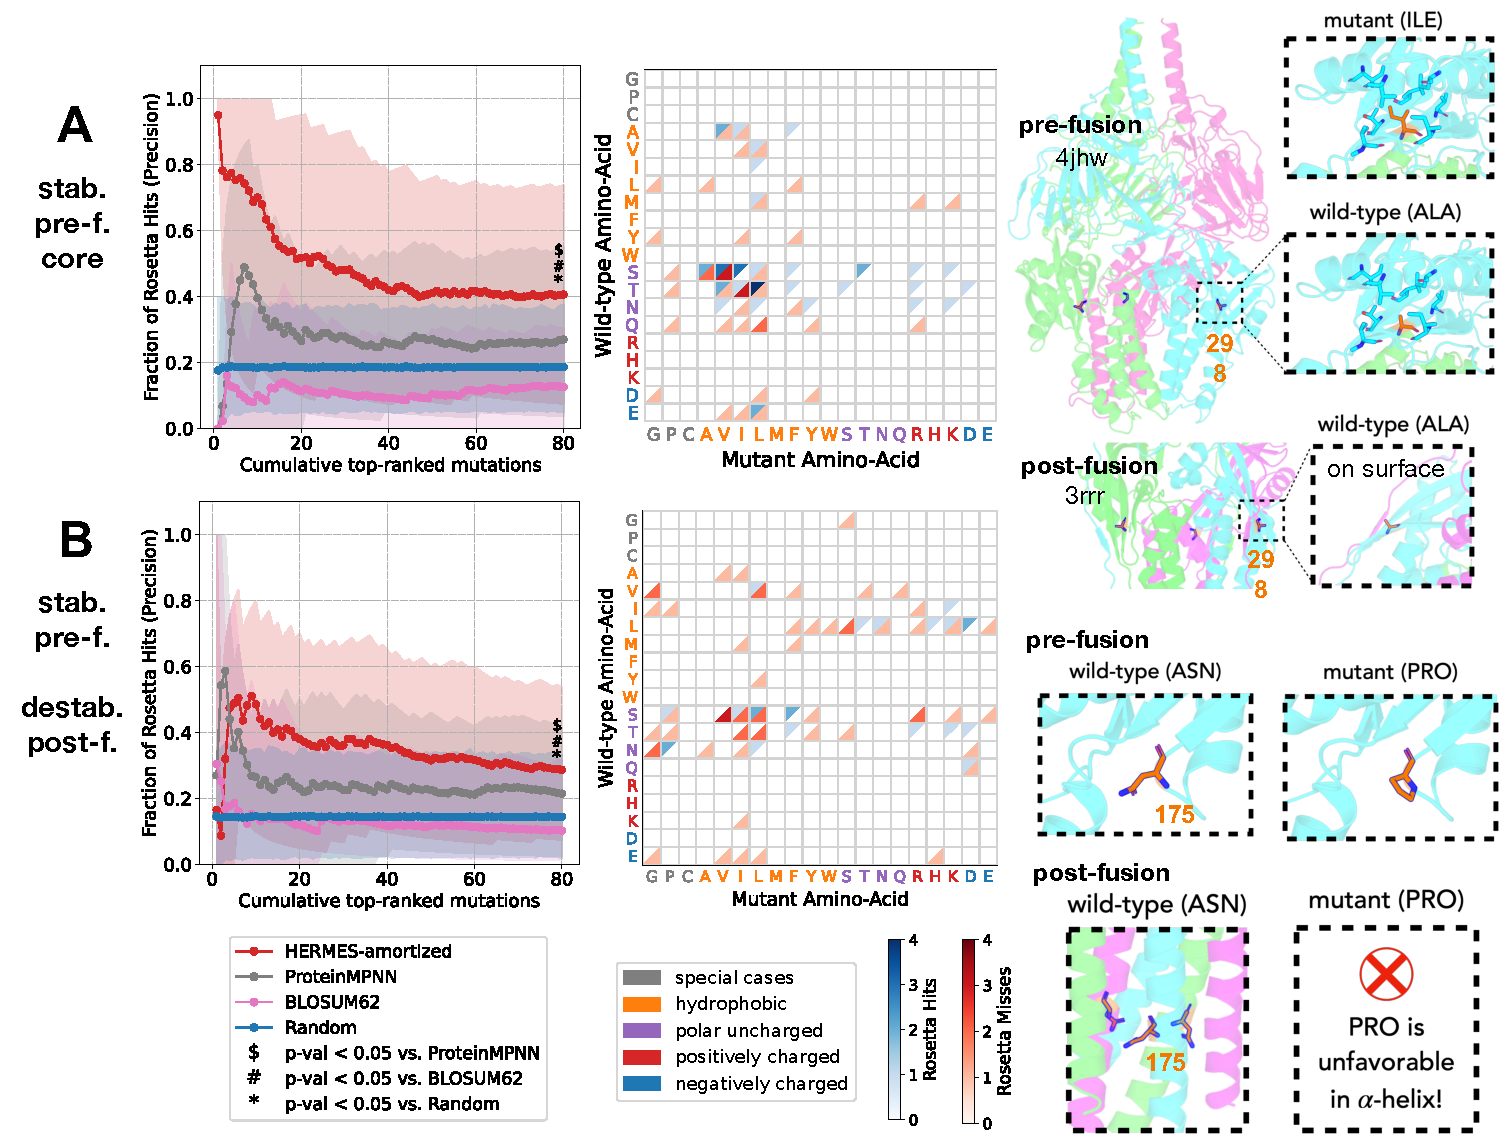
\includegraphics[width=1.0\linewidth]{figures/rsv_f_rosetta_hits_main_figure.pdf}
    \figcaption{\GM{Identifying new antigen-stabilizing mutations with HERMES for RSV-F.}}{
    \GM{
    Panel {\bf A} shows results using the ``stabilize pre-fusion core" pipeline, whereas
    panel {\bf B} shows results using the ``stabilize pre-fusion and destabilize post-fusion" pipeline.
    Each panel is split in three sub-panels.
    \textit{Left}: Rosetta hit rate as a function of number of top-$k$ suggested mutations
    (for all methods except for Random, for which we show the average hit rate of 20 random samples of $k$ mutations from the pool
    of 160 randomly-selected mutations).
    Rosetta hits were computed multiple times via 200 bootstrap samples with replacement of the 50 REU
    scores.
    Solid lines and markers denote the mean across bootstrap samples, whereas shaded regions denote
    the 5-95 percentile range.
    We note that all BLOSUM62 suggestions had a score $\geq 1$ and are ranked by score just like HERMES and ProteinMPNN.
    P-values were computed via Wilcoxon signed-rank test and corrected for multiple testing via
    Bonferroni within each panel.
    \textit{Center}: heatmap showing number of Rosetta hits (blue) and misses (red) for each amino-acid
    mutation pair suggested by HERMES-{\em amortized}.
    Here, Rosetta hits were computed using all 50 REU scores instead of bootstrap samples.
    \textit{Right}: examples of promising antigen-stabilizing mutation identified by each pipeline.
    Mutant structures were generated using PyMOL's protein mutagenesis wizard.
    }
    }
    \label{fig:rsv_f_rosetta_hits_main_figure}
\end{figure}


\begin{table}[t!]
\centering
\begin{tabular}{l | c c | c c}
\toprule
 & \textbf{Per-Struct.} & \textbf{Per-Struct.} & \textbf{Overall} & \textbf{Overall} \\
\textbf{Method} & \textbf{Pearson} & \textbf{Spearman} & \textbf{Pearson} & \textbf{Spearman} \\
\midrule
Rosetta$^*$~\citep{park_simultaneous_2016} & 0.328 & 0.299 & 0.311 & 0.347 \\
FoldX$^*$~\citep{delgado_foldx_2019} & 0.391 & 0.364 & 0.356 & 0.351 \\
\midrule
DDGPred$^*$~\citep{shan_deep_2022} & 0.371 & 0.343 & 0.652 & 0.439 \\
ESM-IF$^*$~\citep{hsu_learning_2022} & 0.231 & 0.209 & 0.296 & 0.287 \\
MIF-Net.$^*$~\citep{luo_rotamer_2022} & 0.395 & 0.348 & 0.667 & 0.480 \\
RDE-Net.$^*$~\citep{luo_rotamer_2022} & 0.469 & 0.433 & 0.642 & 0.527 \\
\midrule
Vanilla Pythia PPI$^\dagger$~\citep{tao_reliable_2025} & 0.478 & 0.449 & 0.709 & 0.537 \\
Pythia-PPI$^\dagger$~\citep{tao_reliable_2025} & 0.565 & 0.527 & 0.785 & 0.637 \\
\midrule
\midrule
\proteinmpnn & 0.281 & 0.282 & 0.331 & 0.315 \\
\proteinmpnnNoise & 0.270 & 0.255 & 0.334 & 0.289 \\
\HERMESPy & 0.306 & 0.287 & 0.285 & 0.272 \\
\HERMESPyNoise & 0.317 & 0.308 & 0.291 & 0.286 \\
\HERMESPyFtRelaxed & 0.231 & 0.241 & 0.290 & 0.242 \\
\HERMESPyNoiseFtRelaxed & 0.222 & 0.239 & 0.276 & 0.222 \\
\HERMESPyFtCdna & 0.347 & 0.331 & 0.380 & 0.342 \\
\HERMESPyNoiseFtCdna & 0.305 & 0.294 & 0.344 & 0.288 \\
\midrule
\HERMESPyFtSkempiEasy & 0.471 & 0.433 & 0.578 & 0.476 \\
\HERMESPyNoiseFtSkempiEasy & 0.430 & 0.389 & 0.512 & 0.420 \\
\HERMESPyFtSkempiMedium & 0.472 & 0.430 & 0.576 & 0.466 \\
\HERMESPyNoiseFtSkempiMedium & 0.407 & 0.368 & 0.497 & 0.403 \\
\HERMESPyFtSkempiHard & 0.435 & 0.398 & 0.395 & 0.380 \\
\HERMESPyNoiseFtSkempiHard & 0.399 & 0.359 & 0.328 & 0.322 \\
\bottomrule
\end{tabular}
\figcaption{Benchmark on predicting mutational effects on protein-protein binding in SKEMPI.}{
The Spearman/Pearson correlations between model-predicted effects of single point mutations and
experimental values from the SKEMPI v2.0 dataset~\citep{jankauskaite_skempi_2019} are reported both
across mutations within each structure individually (``per-structure" correlations), and over
mutations pooled across all complexes (``overall" correlations). Entries marked with $*$ are taken
from ref.~\citep{luo_rotamer_2022} and, for machine learning-based methods (all except Rosetta and
FoldX), were obtained using 3-fold cross-validation over SKEMPI complexes.
Entries marked with $\dagger$ are taken from ref.~\citep{tao_reliable_2025}, and were obtained via
5-fold coss validation on the SKEMPI complex structures.
We evaluate HERMES using three train/test splits defined from SKEMPI metadata, with increasing
difficulty: (i) {\em Easy}, a random split; (ii) {\em Medium}, which groups sites with similar
binding sites (hold-out proteins) into the same split; (iii) {\em Difficult}, which groups sites
from the same held-out protein types (functional classes) into the same split (see Extended Methods,
Appendix~\ref{sec:hermes_appendix} for details).
The HERMES models with most comparable training procedure to the other machine learning models are
those fine-tuned on the \textit{Easy} split, for which we used 3-fold cross-validation with splits
defined by PDB complex.
Note that, similar to HERMES, the machine learning models in ref.~\citep{luo_rotamer_2022} were
fine-tuned on SKEMPI $\Delta\Delta G_{\text{binding}}$ labels only, whereas Pythia-PPI
\citep{tao_reliable_2025} was trained on a mixture of SKEMPI binding labels and FireProtDB stability
labels \citep{stourac_fireprotdb_2021} and further refined via self-distillation.
}
\label{table:skempi_spm}
\end{table}

\subsection{Predicting {binding} effect of mutations}
Predicting the effects of mutations on binding affinity is a central step in target-specific protein
design. In prior work, we demonstrated the utility of HERMES for predicting how mutations in short
peptide antigens alter binding to T-cell receptors in the context of MHC
complexes~\citep{visani_t_2025}. We further leveraged this capability for de novo design of peptide
antigens intended to elicit specific T-cell responses~\citep{visani_t_2025}. Here, we evaluate
HERMES on the single-point mutation effects from the SKEMPI v2.0
dataset~\citep{jankauskaite_skempi_2019}, which spans a substantially broader range of
protein-protein interactions and binding-affinity perturbations.

In a zero-shot setting, HERMES exhibits measurable predictive signal (HERMES-\emph{fixed} 0.50;
Spearman's $\rho = 0.286$). ProteinMPNN achieves comparable overall performance, whereas
physics-based approaches (Rosetta~\citep{chaudhury_pyrosetta_2010} and
FoldX~\citep{schymkowitz_foldx_2005}) perform modestly better (Spearman's $\rho \approx 0.35$). In
contrast to our results for stability prediction, HERMES-\emph{fixed} models correlate more strongly
with binding effects than HERMES-\emph{amortized} models. Interestingly, fine-tuning for stability
(HERMES-\emph{fixed} 0.00+ cDNA117k) yields a slight improvement in binding-effect prediction. A
detailed comparison across models is provided in Table~\ref{table:skempi_spm}.

Next, we fine-tuned HERMES directly on SKEMPI using 3-fold cross-validation. To control for
information leakage under structural similarity, we introduced three homology-aware splitting
strategies of increasing difficulty; the most stringent split prevents complexes from the same
interaction ``class" (e.g., antibody-antigen or TCR-pMHC) from appearing in different folds; see
Extended Methods, Appendix~\ref{sec:hermes_appendix} for details.
Fine-tuned HERMES models achieve substantially stronger correlations, including
under the {\em Difficult} split (Table~\ref{table:skempi_spm}).

Finally, we compared HERMES to recent state-of-the-art methods, RDE-Network and
MIF-Network~\citep{luo_rotamer_2022}, DDGPred~\citep{shan_deep_2022},
ESM-IF~\citep{hsu_learning_2022} and Pythia-PPI~\citep{tao_reliable_2025}. These baselines were also
trained on SKEMPI using 3- or 5-fold cross-validation under protocols analogous, but not identical,
to our {\em easy} split. HERMES fine-tuned on SKEMPI-Easy performs competitively with RDE-Network
and MIF-Network, but trails Pythia-PPI (Table~\ref{table:skempi_spm}). Notably, RDE-Network and
MIF-Network are fine-tuned on SKEMPI $\Delta\Delta G$ labels in a manner similar to our approach,
whereas Pythia-PPI incorporates additional training procedures that further boost performance
(Extended Methods, Appendix~\ref{sec:hermes_appendix}). These procedures are, in principle, applicable
to HERMES as well, but we leave a
systematic evaluation of such extensions, and of HERMES as a general framework for binding-affinity
prediction, to future work.


\section{Summary}

In this chapter, we introduced HERMES, a family of fast, structure-based machine learning models for predicting the
effects of mutations on protein function. HERMES leverages SO(3)-equivariant neural networks
operating on local atomic neighborhoods in a protein structure to predict amino acid propensities,
whose differences can be used to predict mutational effects. This formulation yields a
computationally efficient predictor that is naturally suited to high-throughput settings. HERMES
captures mutational impacts on diverse phenotypes, including thermodynamic stability and
protein-protein binding affinity, and it provides a practical tool for antigen stabilization in
vaccine design.

A central finding is that encoding packing flexibility is essential for accurate predictions across
mutations involving amino acids of different sizes. HERMES-{\em fixed}, a lightweight protocol that
evaluates mutations in the rigid wild-type structure, exhibits strong bias toward size-conserving
substitutions. Explicitly modeling relaxation via Rosetta~\citep{chaudhury_pyrosetta_2010},
(HERMES-{\em relaxed} protocol) resolves this bias but incurs substantial computational cost. Our
amortized approach offers an effective compromise: by fine-tuning on relaxed predictions for just
0.5\% of pre-training data, HERMES-{\em amortized} learns implicit packing flexibility that can be
leveraged for predictions at HERMES-{\em fixed} speed. This capability proves particularly valuable
for antigen stabilization, where HERMES-{\em amortized} recovers over half of the verified
stabilizing mutations in our benchmark and shows strong performance on proline substitutions (87.5\%
recovery), which stabilize proteins by restricting backbone conformational freedom.

Beyond zero-shot use, HERMES can be fine-tuned directly on experimental labels using a simple
end-to-end procedure. Notably, both the native and the fine-tuned models use the difference of amino
acid scores for predicting mutational effects, which yields an inherent reversibility with respect
to mutation order--a thermodynamic consistency property that is often enforced via explicit
19$\times$ data augmentation~\citep{diaz_stability_2024}.

With fine-tuning, HERMES achieves competitive accuracy on thermodynamic stability benchmarks when
trained on the same data as prior methods~\citep{blaabjerg_rapid_2023, diaz_stability_2024,
dieckhaus_transfer_2024}. Interestingly, stability fine-tuning does not consistently transfer to
antigen stabilization and can even degrade performance. One plausible explanation is dataset
mismatch: the high-throughput stability datasets used for
fine-tuning~\citep{tsuboyama_mega-scale_2023} are enriched for relatively small, compact domains,
whereas vaccine antigens are often larger, multi-domain, and conformationally heterogeneous, with
stabilizing mutations frequently targeting quaternary contacts, glycoprotein-specific features, or
prefusion-state constraints. Resolving this discrepancy will likely require broader supervision that
better reflects antigen structure and design objectives, or task-aligned fine-tuning data.

We also demonstrate that pre-training on wild-type amino acid classification remains necessary for
strong performance; models trained only on currently-available experimental stability data fail.
Notably, pre-trained models exhibit ``wild-type preference," assigning elevated probabilities to
wild-type residues in wild-type structural contexts. This bias correlates with sequence similarity
to pre-training proteins, suggesting partial memorization rather than purely generalizable learning.
Fine-tuning partially ameliorates but does not eliminate this effect, representing a fundamental
trade-off in current training paradigms. More robust pre-training objectives, stronger
regularization, or explicit debiasing strategies may be required to fully address this issue.

A key application we highlight is structure-based vaccine design, where practitioners seek to
stabilize substitutions that preserve a desired prefusion conformation of a vaccine antigen to
elicit immune responses targeting relevant epitopes. For this task, a useful model should propose
stabilizing mutation candidates across different sites of an antigen.
On the limited available data comprising 33 verified antigen-stabilizing mutations across five viruses,
HERMES performs well in recovering these mutations.
\GM{We also develop two pipelines to suggest mutations with HERMES across the full antigen,
showing close agreement with predictions made with the physics-based model Rosetta, which we
suggest to use to further filter the candidate set of mutations.}
Moreover, the strict locality of the model makes it straightforward and
fast to apply to large antigens and assemblies that can pose challenges for architectures modeling
global interactions in proteins.
Our results show that local all-atom environments modeled by HERMES
can encode multiple stabilization mechanisms, including cavity filling, post-fusion disruptions and
pre-fusion backbone rigidification via prolines, and favorable electrostatic remodeling,
while also underscoring limitations for mechanisms
that depend on long-range coupling, or multi-site epistasis.


We further evaluated HERMES on predicting changes in protein--protein binding affinity using the
SKEMPI dataset~\citep{jankauskaite_skempi_2019}. In the zero-shot setting, HERMES shows measurable
predictive signal, and supervised fine-tuning on SKEMPI {substantially} improves performance.
Recent state-of-the-art approaches for binding prediction like Pythia-PPI~\citep{tao_reliable_2025}
indicate that design choices such as self-distillation can substantially improve
performance~\citep{tao_reliable_2025}; we expect HERMES would similarly benefit from such
approaches, representing a clear next step.

Several directions could extend HERMES' capabilities. Developing larger, more diverse training
datasets, particularly for antigen stabilization and binding, would likely improve performance, as
our results indicate that training data dominates architectural differences in determining benchmark
performance. The locality of HERMES appears to be a double-edged sword: local neighborhoods reduce
input complexity, remove constraints on protein size, and improve scalability, but necessarily limit
the model's ability to capture long-range epistasis and allosteric coupling. We view HERMES as a
hypothesis-generation tool whose predictions are most reliable when mutational effects are driven
primarily by short-range interactions and local packing. Productive directions for future work
include better characterizing when locality suffices, further reducing pre-training-induced biases,
and developing multi-scale approaches that efficiently combine local all-atom predictors with
complementary global or multi-site models to capture mechanisms beyond the local neighborhood.

